\documentclass[english,a4paper,anonymous,cleveref,thm-restate]{lipics-style/lipics-v2021}
\pdfoutput=1 %% as indicated in the authors guideline

\input{macros}


%% PC members that may understand the paper
%% Davide Sangiorgi
%% Michele Boreale
%% Daniele Gorla
%% Valeria Vignudelli
%% Alexandra Silva



\newcommand{\ie}{{\em i.e.}\xspace}
\newcommand{\sts}[2]{\ensuremath{\langle #1, #2 \rangle}}
\newcommand{\myspace}{\phantom{\scalebox{.6}{$\ok$}}}
\newcommand{\ltsof}[1]{\ensuremath{\textsc{lts}(#1)}}
\newcommand{\ltsFWof}[1]{\ensuremath{\textsc{ltsFW}(#1)}}


\renewcommand{\traceA}{s_1}
\newcommand{\traceB}{s_2}
\newcommand{\traceC}{s_3}


\DeclareUnicodeCharacter{2208}{$\in$}
\DeclareUnicodeCharacter{2203}{$\exists$}
\DeclareUnicodeCharacter{2200}{$\forall$}
\DeclareUnicodeCharacter{2113}{$\ell$}
\DeclareUnicodeCharacter{03B1}{$\alpha$}
\DeclareUnicodeCharacter{27F6}{$\longrightarrow$}
\DeclareUnicodeCharacter{2227}{$\wedge$}
\DeclareUnicodeCharacter{2228}{$\vee$}
\DeclareUnicodeCharacter{2261}{$\equiv$}
\DeclareUnicodeCharacter{3BC}{$\mu$}
\DeclareUnicodeCharacter{2260}{$\neq$}
\DeclareUnicodeCharacter{27F9}{$\Longrightarrow$} %⟹ (U+27F9)
\DeclareUnicodeCharacter{03B7}{$\eta$} %η (U+03B7)
\DeclareUnicodeCharacter{03BB}{$\lambda$} %λ (U+03BB)
\DeclareUnicodeCharacter{03C4}{$\tau$} %λ (U+03BB)
\DeclareUnicodeCharacter{21D3}{$\Downarrow$}
\DeclareUnicodeCharacter{227C}{$\preccurlyeq$} %λ (U+03BB)
\DeclareUnicodeCharacter{2081}{${}_1$} %λ (U+03BB)
\DeclareUnicodeCharacter{2082}{${}_2$} %λ (U+03BB)
\DeclareUnicodeCharacter{2091}{${}_{\textrm{e}}$} %λ (U+03BB)
\DeclareUnicodeCharacter{219B}{$\nrightarrow$} %λ (U+03BB)
\DeclareUnicodeCharacter{2286}{$\subseteq$} %λ (U+03BB)
\DeclareUnicodeCharacter{2291}{$\sqsubseteq$} %λ (U+03BB)
\DeclareUnicodeCharacter{2205}{$\emptyset$} %λ (U+03BB)
\DeclareUnicodeCharacter{227E}{$\precsim$} %λ (U+03BB)
\DeclareUnicodeCharacter{25B7}{$\triangleright$} %λ (U+03BB)
\DeclareUnicodeCharacter{2194}{$\leftrightarrow$} %λ (U+03BB)
\DeclareUnicodeCharacter{2250}{$\doteq$} %λ (U+03BB)
\DeclareUnicodeCharacter{228E}{$\uplus$} %λ (U+03BB)
\DeclareUnicodeCharacter{27FF}{$\rightsquigarrow$} % ⟿
\DeclareUnicodeCharacter{22CD}{$\simeq$} %
\DeclareUnicodeCharacter{2216}{$\setminus$} %
\DeclareUnicodeCharacter{2093}{$_x$} %
\DeclareUnicodeCharacter{2913}{$\downarrow_i$} %
\DeclareUnicodeCharacter{22D6}{$\lessdot$} %

\newcommand{\mspreorder}{\ensuremath{\preceq_{MS}}}
\newcommand{\aspreorder}{\ensuremath{\preceq_{AS}}}
\newcommand{\outof}[1]{O(#1)}
\newcommand{\outnorm}[2]{\mathit{strip}(#1, #2)}
\newcommand{\outputmultisetSym}{\mathsf{mbox}}
\newcommand{\outputmultiset}[1]{\outputmultisetSym(#1)}


\title{Constructive characterisations of the
  \texorpdfstring{\mustpreorder}{MUST-preorder} for asynchrony}


%%% FORMAT
%%% \author{name}{affil}{email}{orcid}{funding}.


  \author{ANONYMOUS}{HIDDEN}{}{}{}
% \author{Giovanni Bernardi}{IRIF}{gio@irif.fr}{ORCID}{F}
%
% \author{Ilaria Castellani}{INRIA}{mail}{ORCID}{F}
%
% \author{Paul Laforgue}{Nomadic Labs}{mail}{ORCID}{F}
%
% \author{Léo Stefanesco}{Max Planck}{mail}{ORCID}{F}
%
% \authorrunning{G. Bernardi, I. Castellani, P. Laforgue, and L. Stefanesco}

\ccsdesc{classification}

%% \acknowledgements{
%%   This paper benefited from discussions with Guillaume Geoffroy, Hugo Herbelin and Pierre-Evariste Dagand.
%% }

\begin{document}
\maketitle

\begin{abstract}
  De Nicola and Hennessy's \mustpreorder is a contextual refinement which states
that a server~$\serverB$ refines a server~$\serverA$ if all clients satisfied
by~$\serverA$ are also satisfied by~$\serverB$. Owing to the universal
quantification over clients, this definition does not yied a practical proof
method for the \mustpreorder,  %does not enjoy a simple proof method, and
and alternative characterisations are necessary to reason on it.

We present the first characterisations of the \mustpreorder
that are constructive, supported by a mechanisation in Coq,
and independent from any calculus:
our results pertain to Selinger output-buffered
agents with feedback. This is a class of Labelled Transition Systems
that captures programs that communicate asynchronously via
a shared unordered buffer, as in
% \ila{the asynchronous variants of
%   \CCS and the $\pi$-calculus.}
{asynchronous \CCS or the
asynchronous $\pi$-calculus.}

Our results are surprising: the behavioural characterisations
devised for synchronous communication carry over as they stand
to asynchronous communication, if servers are enhanced to act as forwarders,
\ie they can input any message as long as they
store it back into the shared buffer.
This suggests a technique to port standard characterisations
%\gb{and also failure refinement}
from synchronous to asynchronous settings.
\end{abstract}


\section{Introduction}
\label{sec:intro}
Code refactoring is a routine task to develop or update software, and
it requires methods to ensure that a program~$\serverA$ can be safely
replaced by a program~$\serverB$.  One way to address this issue is
via refinement relations, \ie preorders.  For programming languages,
the most well-known one is Morris \emph{extensional} preorder
\cite[pag.~$50$]{morris}, defined by letting~$p \leq q$ if for all
contexts~$C$, whenever~$C[p]$ reduces to a normal form~$N$,
then~$C[q]$ also reduces to~$N$.



{\bfseries Comparing servers.}
This paper studies a version of Morris preorder for
\nondeterministic asynchronous \svrclt systems.
In this setting it is natural to reformulate the preorder by replacing
reduction to normal forms (\ie termination) with a suitable
\emph{liveness} property.
Let~$\csys{ \server }{ \client }$ denote a {\em \svrclt\ system},
that is a parallel composition in which the identities of the
server~$\server$ and the client~$\client$ are distinguished, and
whose computations have the form
$
\csys{\server~}{~\client} =
\csys{ \server_0 }{ \client_0 } \st{ }
\csys{ \server_1 }{ \client_1 } \st{ }
\csys{ \server_2 }{ \client_2 } \st{ } \ldots,
$
where each step represents either an internal computation
of one of the two components, or an interaction between them.
Interactions correspond to handshakes, where
two components ready to perform matching input/output actions
advance together.
We express liveness by saying that  $\server \text{ \emph{must pass} }
\client$, denoted $\Must{ \server }{ \client }$, if in every maximal
computation of $\csys{ \server }{ \client
}$ there exists a state $\csys{ \server_i}{ \client_i}$ such that
$\good{\client_i}$, where~$\goodSym$ is a decidable predicate
 indicating that the client has reached a successful state.
Servers are then compared according to their capacity to
satisfy clients, \ie via contexts of the form~$\csys{[-]}{\client}$
and the predicate~$\opMust$.
%namely to lead clients to successful states, \ie via
%In other words, servers are compared
%via contexts of the form~$\csys{[-]}{\client}$.
%, as argued also by \cite{DBLP:phd/us/Thati03}.
Morris preorder %, when restricted to computations leading to
%successful states,
then becomes the \mustpreorder\
by De Nicola and Hennessy~\cite{DBLP:journals/tcs/NicolaH84} :
%\begin{equation}
%  \label{eq:must-preorder}
%%
$
  \serverA \testleqS \serverB \text{ when } \forall \client \wehavethat
  \Must{\serverA}{\client} \implies
  \Must{\serverB}{\client}.
  $
%%\end{equation}


  {\bfseries Advantages.}
  The \mustpreorder is by definition liveness preserving,
  because $\Must{ \server }{ \client }$ literally means that
  ``in every execution something good must happen (on the client
  side)''.  Results on~$\testleqS$ thus shed light on
  liveness-preserving program transformations.

  The~\mustpreorder is independent of any particular calculus,
  as its definition requires simply
  (1) a reduction semantics for the parallel composition
  $\csys{ \server }{ \client }$, and (2)
  a predicate $\goodSym$ over programs.
  %%% LONG VERSION
  %% We thus do not fix any particular calculus:
  %% we assume a way of describing how servers and clients interact
  %% with the environment, and use it to define the semantics of $\csys{
  %%   - }{ - }$.
  %%As a result,
  Hence~$\testleqS$
  % the relation~$\testleqS$
  % lets us compare software components
  may relate servers written in different languages. For instance, servers written in
  \textsc{OCaml} may be compared to servers written in \textsc{Java}
  according to clients written in \textsc{Python}, because all these
  languages communicate using the same basic protocols.
  %%VERY DODGY STATEMENT:  that we are able to model.

  {\bfseries Drawback.}
  The definition of the \mustpreorder is {\em contextual}: proving that
  $\serverA~\testleqS~\serverB$ requires analysing an {\em
  infinite} amount of clients, and so the definition of
the preorder does not entail an effective proof method.
A solution to this problem is to define an {\em alternative (semantic)
  characterisation} of the preorder~$\testleqS$, \ie a
preorder~$\altleq$ that coincides with~$\testleqS$
and does away with the universal quantification over clients (\ie contexts).
In {\em synchronous} settings, i.e. when both input and output
actions are blocking, such alternative characterisations have been thoroughly
investigated, %for instance
typically via a behavioural approach.






\begin{figure}[t]
  \hrulefill
  \begin{center}
    \begin{minipage}{4cm}
        \centering
      \begin{tikzpicture}
        \node[state,scale=0.8] (s1) at (6,0) {$\server_0$};
        \node[state,scale=0.8,below of=s1,left of=s1] (s2) {$\server_1$};
        \node[state,scale=0.8,below of =s1,right  of=s1] (s3) {$\server_2$};
        \node[state,scale=0.8,below of=s2] (s4) {$\server_3$};
        \node[state,scale=0.8,below of=s3] (s5) {$\server_4$};

        \node[scale=0.8, below of = s5] (dummy) {$$};

        \path[->]
        (s1) edge node [above left,scale=0.8] {$\texttt{str}$} (s2)
        (s1) edge node [above right,scale=0.8] {$\texttt{float}$} (s3)
        (s2) edge node [left,scale=0.8] {$\co{\texttt{int}}$} (s4)
        (s3) edge node [right,scale=0.8] {$\co{\texttt{long}}$} (s5);
      \end{tikzpicture}
      \end{minipage}%
      \begin{minipage}{4cm}
        \centering\vskip-0.95em
      \begin{tikzpicture}
        \node[state,scale=0.8] (s0) at (0,0) {$\client_0$};
        \node[state,dashed,scale=0.8,below right = +15pt and +15pt of s0] (s1) {$\client_2$};
        \node[state,scale=0.8,below left = +15pt and +15pt of s0] (s2) {$\client_1$};
        \node[state,dashed,scale=0.8,below right = +15pt and +15pt of s2] (s3) {$\client_3$};

        \path[->]
        (s0) edge node [above left,scale=0.8] {$\co{\texttt{str}}$} (s2)
        (s0) edge node [above right,scale=0.8] {$\texttt{int}$} (s1)
        (s2) edge node [below left,scale=0.8] {$\texttt{int}$} (s3)
        (s1) edge node [below right,scale=0.8] {$\co{\texttt{str}}$} (s3);
    \end{tikzpicture}
  \end{minipage}
  \end{center}
  \vskip-1.5em
  \caption{The behaviours of a server $\server_0$ and of a client $\client_0$.}
  \label{fig:first-example}
  \hrulefill
\end{figure}



{\bfseries Behavioural characterisations.}
Alternative preorders %that capture~$\testleqS$
are usually
defined % as follows
in two steps:
%
- First, programs are associated with labelled transition systems (LTSs)
% such as the ones
like those in \rfig{first-example}, where transitions are
labelled by input actions such as $\texttt{str}$, %$\aa$,
output actions such as $\co{\texttt{str}}$, or the internal action
$\tau$ %(not featured in~Figure~\ref{fig:first-example}),
while dotted nodes represent successful states, \ie
those satisfying the predicate~$\goodSym$.
There, the server~$\server_0$ is ready to input either a string or a
float.
  %, and it is the environment that, by offering an output of
 % either type, will make~$\server$ move to either~$\server_1$
 % or~$\server_2$.
  The client~$\client_0$, on the other hand, is ready to either output
  a string, or input an integer. The input ${\tt int}$ makes the
  client move to the %$\goodSym$
  successful state~$\client_2$, while the output
  $\co{\tt{str}}$ makes the client move to the state $\client_1$, where it can
  still perform the input ${\tt int}$ to reach the %$\goodSym$
  successful state~$\client_3$. Output transitions enjoy a
  sort of %diamond property
  commutativity property on which we will return later.
  Programs $\serverA, \serverB, \client, \ldots$ are usually
  associated with their behaviours via inferences rules, which
  implicitly define a function $\ltsof{ - }$ that, given a
  program~$\server$, returns the LTS whose root is~$\server$.\\
  %%%%% END EXPLANATION EXAMPLE LTS IN FIG. 1
%
%  \noindent  
- Second, program behaviours, \ie~LTSs, are used to define the
alternative preorders for~$\testleqS$ %via
following one of two different
approaches: \MustSets or \AcceptanceSets.


{\bfseries Alternative preorders for synchrony.}  Both approaches were
originally proposed for % Milner's
% the Calculus of Communicating Systems ($\CCS$)
the calculus \CCS~\cite{DBLP:books/daglib/0098267},
where communication is synchronous.
The first alternative preorder, which we denote by~$\msleq$, was put
forth by De Nicola~\cite{DBLP:journals/tcs/NicolaH84}, and it
compares server behaviours according to their \MustSets, \ie~the sets of
actions that they may perform.
The second alternative preorder, which we denote by~$\asleq$, was put
forth by Hennessy~\cite{DBLP:books/daglib/0066919}, and it compares the
\AcceptanceSets of servers, \ie~how servers can be moved out of their
potentially deadlocked states.
Both these preorders characterise~$\testleqS$ in the
  following sense:
%In this case the characterisation is as follows,
%\ila{``In this case, the characterisation is:''}}
%Theorem 4.4.6 of \cite{DBLP:books/daglib/0066919} states the following
%characterisation: \ilacom{Do not mention the theorem, write simply
\begin{align}
      \label{eq:bhv-mustset-characterisation}
  \forall \serverA , \serverB \in \CCS \wehavethat & \serverA \testleqS \serverB
  \text{ iff } \ltsof{\serverA} \msleq \ltsof{\serverB}
  \\
    \label{eq:bhv-accset-characterisation}
  \forall \serverA , \serverB \in \CCS \wehavethat & \serverA \testleqS \serverB
  \text{ iff } \ltsof{\serverA} \asleq \ltsof{\serverB}
\end{align}

%% \gb{%
%% {\smaller[.99]
%% $$
%% \begin{array}{|l@{\hskip 1pt}l@{\hskip 2pt}c@{\hskip 2pt}l|l@{\hskip 1pt}l@{\hskip 2pt}c@{\hskip 2pt}l|}
%%   \hline
%%   \forall \serverA , \serverB \in \CCS \wehavethat & \serverA \testleqS \serverB
%%   & \text{ iff } & \ltsof{\serverA} \asleq \ltsof{\serverB}
%%   &
%%    \forall \serverA , \serverB \in \obaFB
%%     \wehavethat& 
%%     \serverA \testleqS \serverB
%%     &\text{ iff }&
%%     \liftFW{\serverA} \msleq \liftFW{\serverB}
%% \\
%%   \label{eq:bhv-mustset-characterisation}
%%   \forall \serverA , \serverB \in \CCS \wehavethat & \serverA \testleqS \serverB
%%   & \text{ iff } & \ltsof{\serverA} \msleq \ltsof{\serverB}
%%   &
%%   \forall \serverA , \serverB \in \obaFB
%%     \wehavethat&
%%     \serverA \testleqS \serverB
%%     &\text{ iff }&
%%     \liftFW{\serverA} \asleq \liftFW{\serverB}
%%     \\[2pt]
%%     \hline
%%     \multicolumn{4}{c}{\text{(a) Seminal results}}
%%     &
%%     \multicolumn{4}{c}{\text{(b) Novel results}}
%% \end{array}
%% $$
%% }
%% }%% \gb

%For instance \cite{DBLP:journals/iandc/BorealeNP02} use it
%in an asynchronous settings, \ilacom{I would not mention asynchronous
%  approaches here. I would only do it after we start talking about the
%  asynchronous case, namely after the paragraph ``On the Internet,
%  though\ldots''} and
%% REDUNDANT FOR WE ALREADY SAID IT ABOVE
%% In both~(\ref{eq:bhv-accset-characterisation}) and~(\ref{eq:bhv-mustset-characterisation}),
%% $\CCS$ is Milner's Calculus of Communicating Systems
%% \cite{DBLP:books/daglib/0098267}, and thus~$\serverA$ and~$\serverB$
%% are syntactic terms.
%%   There the server~$\server$ is \ila{initially} in a {\em stable state}: it
%% cannot perform any $\tau$ move, but \ila{it} is ready to input either a string
%% or a float, and it is the environment that, by offering an output of
%% either type, will make~$\server$ move to a different state.
%% Hence,~$\server_0$ models an {\em external} choice. The
%% client~$\client$, on the other hand, can either output a string, or
%% move to a different state via an internal computation.
%This is a form of {\em internal choice}. \ilacom{To my view, this does
%  not represent an internal choice - which should have both outcoming
%  transitions labelled by $\tau$ - but rather a parallel composition
%  of the output $\co{\texttt{str}}$ with the action $\tau$, as
%  witnessed by the fact that the LTS is diamond shaped (cf axiom
%  \ila{\outputtau).}}
%can interact
  %In either case, in each maximal computation of $\csys{ \server }{ \client }$ the client will eventually reach a successful state.}

%%%%%%%%% ILARIA: Logical characterisation, commented off 23/11/23

% {\em Logical} characterisations of~$\testleqS$, instead,
% require defining when a program~$\server$ models a certain
% formula~$\phi$, denoted $\server \models \phi$, where
% formulae belong typically to the recursive Hennessy-Milner
% logic, \ie the modal $\mu$-calculus, and the
% characterisations essentially identify the fragment~$L$
% of this logic, which is necessary and sufficient to capture
% the contextual preorder:
% \begin{equation}
%   \label{eq:logical-characterisation}
%   \forall \serverA , \serverB \in \CCS \wehavethat
%   \serverA \testleqS \serverB
%   \text{ iff }  (\forall \phi \in L \wehavethat \serverA \models \phi \implies \serverB \models \phi)
% \end{equation}
% These characterisations, given in Theorem 4.1 by
% \cite{DBLP:journals/jacm/AcetoH92} and indirectly by
% \cite{DBLP:journals/corr/abs-1011-6438},
% %are close in spirit to the
% %well-known theorem by \cite{DBLP:journals/jacm/HennessyM85},  and they
% identify the behavioural proprieties that are invariant under code refactoring done via~$\testleqS$.

%% OLD POPL TEXT
%% By contrast, {\em logical} characterisations
%% define~$\altleq$~comparing servers according to the formulae of the
%% recursive Hennessy-Milner logic\footnote{\ie the modal $\mu$-calculus}
%% that they satisfy: %
%% if $\serverA \altleq \serverB$ and~$\serverA$~satisfies a
%% formula~$\phi$,
%% %such %as~$\dmd{\texttt{str}}(\dmd{\texttt{int}}\true
%% % \wedge \dmd{\texttt{float}}\true)$
%% then~$\serverB$~also does.

%%%%%%%%% ILARIA: end of Logical characterisation %%%%%%%%%%%%%%%





{\bfseries Asynchrony.} %
In distributed systems, however,
communication is inherently asynchronous. For instance, the standard TCP
transmission on the Internet is asynchronous.
Actor languages like \textsc{Elixir} and \textsc{Erlang}
implement asynchrony via mailboxes, and both \textsc{Python} and
\textsc{JavaScript} offer developers the constructs
\textsc{async/wait}, to return promises (of results) or wait for
them.
In this paper we model asynchrony via \emph{output-buffered agents with
feedback}, as introduced by Selinger~\cite{DBLP:conf/concur/Selinger97}.
These are LTSs obeying the axioms in \rfig{axioms}, where~$\aa$ denotes
an input  action,~$\co{\aa}$ denotes an output  action,~$\tau$ denotes
the internal action, and~$\alpha$ ranges over all these actions.
For instance, the \outputcommutativity axiom states that an
output $\co{a}$ % $\co{a}$ that is followed by any action~$\alpha$,
can always be postponed: if $\co{a}$ is followed by any action~$\alpha$,
it can commute with it.
In other terms, outputs are
non-blocking,as illustrated by the LTS for~$\client_0$ in \rfig{first-example}.

\input{axioms-figure}

%The \outputfeedback axiom states that any message emitted by an agent
%is immediately available as input to the agent itself.

%% These axioms are typically enjoyed by LTS of calculi in which
%% communication takes place via a global unordered mailbox.
%% In turn, this communication model is the one that a priori allows for the most
%% \nondeterminismT, and this is why we favour it.


%% gb{The~$\tau$ action denotes internal computation of an agent, or a
%%   interactions between two agents. For instance, the computations
%%   in the system~$\csys{ \server_0 }{ \client_0 }$, where~$\server_0$
%%   and~$\client_0$ are give in \rfig{first-example} amount to
%%   $\csys{ \server_0 }{ \client_0 } \st{\tau}
%%   \csys{ \server_1 }{ \client_2 } \st{\tau} \csys{ \server_3 }{
%%   \client_3 }$.
%%   Note that \outputcommutativity implies a lack of causality between
%%   the client output $\co{{\tt str}}$ and its input ${\tt int}$, and hence
%%   the order of interactions depends on the order of the inputs in the
%%   server side.}
%%% NOT IMPORTANT ON A FIRST READ
%% We find it worth attention for it is the one that allows for the most
%% \nondeterminismT, and thus proofs that tackle this model can be adapted to more
%% deterministic settings, for instance when asynchrony is implemented
%% via ordered queues, as in \cite{josephs}.
%% The more deterministic the semantics, the easier the reasoning,
%% as already shown by theories of \mustpreorder in \CCS as compared
%% to the ones for session types \cite{DBLP:journals/mscs/BernardiH16}.
%% In output-buffered agents, outputs enjoy the \outputcommutativity\ and

%% \outputfeedback\ axioms.
{\bfseries Theoretical issues.} % due to asynchrony.}
The practical importance of asynchrony motivates a % suitable
specific study of~$\testleqS$. Efforts in this direction have
already been made, all of which focussed on process calculi
\cite{DBLP:conf/fsttcs/CastellaniH98,DBLP:journals/iandc/BorealeNP02,DBLP:phd/us/Thati03,DBLP:journals/jlp/Hennessy05}.
% The axioms in \rfig{axioms}, though, create an asymmetry between output
% and input actions, because they % force
% impose properties only over the outputs.
Note that the  axioms in \rfig{axioms} impose conditions
  only over outputs. This asymmetric treatment of inputs and outputs
substantially complicates the proofs of completeness and soundness of
the alternative characterisations of~$\testleqS$.
%% LONG VERSION
%% For instance, the phenomenon leaps out in the completeness proofs of alternative
%% characterisations, for their arguments depend on the contexts (\ie
%% clients), and the standard reasoning requires clients with blocking
%% outputs, that do not exist in the asynchronous setting.  As a
%% consequence, the results in (\ref{eq:bhv-mustset-characterisation})
%% and (\ref{eq:bhv-accset-characterisation}) do not hold in settings
%% where programs communicate by modifying a shared unordered buffer
%% \cite{DBLP:conf/concur/Selinger97,DBLP:conf/ecoop/HondaT91,
%%   boudol:inria-00076939}.
% and hence outputs are {\em non-blocking}.
%% For instance, \cite{DBLP:conf/fsttcs/CastellaniH98}
%% give simple counterexamples to~(\ref{eq:bhv-accset-characterisation})
%% in the setting of asynchronous \CCS (ACCS). There $ {\tt str}.\Nil
%% \testleqS \Nil $, \ie a server that does nothing is as good as a
%% server than can input a  string, while $ {\tt str}.\Nil \not \asleq
%% \Nil $.
%As for
To underline the subtleties due to asynchrony, we note that the completeness
result for asynchronous
  \CCS given by Castellani and Hennessy
  in~\cite{DBLP:conf/fsttcs/CastellaniH98},
  and subsequently extended to the $\pi$-calculus by 
  Hennessy~\cite{DBLP:journals/jlp/Hennessy05},
  is false (see \rapp{counterexample}).

% the technical work to obtain
% completeness (lemmas 3.26 and 3.27 there) to the reader.
%% LONG VERSION
%% Similarly
%% for Theorem 5.3 of \cite{DBLP:phd/us/Thati03}, which is presented as
%% a ``simple adaptation of the [\ldots] characterisation [\ldots] over
%% asynchronous CCS \cite{DBLP:conf/fsttcs/CastellaniH98}'', and
%% therefore not provided with a proof.  Instead,
%% \cite{DBLP:journals/iandc/BorealeNP02} change the definition of the
%% alternative preorder to arrive at a characterisation.


%% \footnote{It should be noted also that the behavioural preorder of
%% \cite{DBLP:conf/fsttcs/CastellaniH98} relies on acceptance sets,
%% while the one given in  \cite[Definition 5.8]{DBLP:phd/us/Thati03}
%% relies on $\Must$-sets, so anyhow the proof of Theorem 5.3 should not
%% follow from the one by Castelanni and Hennessy, but rather from the
%% one of \cite{DBLP:journals/iandc/BorealeNP02}.}.
%%%%%%%%% ILARIA: moved earlier 23/11/23 %%%%%%%%%%%%%%%%%%%
% On the Internet, though, communication is {\em asynchronous}, because so is
% the standard TCP transmission; actor languages like
% \textsc{Elixir} and \textsc{Erlang} implement asynchrony via mailboxes, and
% both \textsc{Python} and \textsc{Javascript} offer developers the \textsc{async/wait}
% constructs, to return promises (of results) or to wait for them.
% The reality is thus in stark contrast with the state in which the
% existing theory of~$\testleqS$ lays, and calls for a solid study of
% this preorder in an asynchronous setting, via tools fit to make us
% tame the lengthy (and at times tedious) proofs about semantics of
% programming languages.
% To provide such a foundation, we mechanise our work in the Coq proof
% assistant.
%%%%%%%%%%%%%%%%%%%%%%%%%%%%%%%%%%%%%%%%%%%%%%%%%%%



{\bfseries Contributions and paper structure.} Our main contributions
may be summarised as follows
  (where for each of them, we detail where it is presented):
%\ilacom{I would first give the contributions and then shortly describe
%  the paper structure at the end.}
\begin{itemize}
\item 
The first behavioural
characterisations of the \mustpreorder (\rthm{testleqS-equals-accleq},
\rthm{testleqS-equals-mustsetleq}), that are {calculus independent}, in
that both our definitions and our proofs work directly on LTSs.
%\leo{not just proofs, the statements too!}
%% NOT USEFULL HERE. GET TO THE POINT, FAST.
%% The only hypothesis we use is that
%% the servers at hand satisfy the axioms for output buffered agents
%% proposed by \cite{DBLP:conf/concur/Selinger97}, plus additional
%% two to obtain completeness.
%% These axioms for asynchrony allow the largest amount of
%% \nondeterminism in LTS, so our results hold in arguably
%% the most complex scenario wrt. message-passing.
Contrary to all the previous works on the topic, we show that the {\em
  standard} alternative preorders characterise the~\mustpreorder also
in Selinger asynchronous setting.  To this end, it suffices to
enrich the server semantics with {\em forwarding}, i.e. ensure that
servers are ready to receive any input message, as long as they store
it back in a global shared buffer. This idea, although we use it here in a slightly
different form, was pioneered by Honda et al.~\cite{DBLP:conf/ecoop/HondaT91}.
In this paper we propose a construction that works on any LTS (\rlem{liftFW-works})
and we show the following counterparts of Equations
(\ref{eq:bhv-mustset-characterisation}) and
(\ref{eq:bhv-accset-characterisation}),
where $\obaFB$ denotes the LTSs of output-buffered agents with
  feedback, and~$\liftFWSym$ is the function that enhances them with forwarding:
\begin{align}
  \forall \serverA , \serverB \in \obaFB
    \wehavethat&
    \serverA \testleqS \serverB
    \text{ iff }
    \liftFW{\serverA} \msleq \liftFW{\serverB}
    \tag{a}
    \\
\forall \serverA , \serverB \in \obaFB
    \wehavethat&
    \serverA \testleqS \serverB
    \text{ iff }
    \liftFW{\serverA} \asleq \liftFW{\serverB}
    \tag{b}
\end{align}

%% \begin{equation}
%%   \begin{array}{ll}
%%     \forall \serverA , \serverB \in \obaFB
%%     \wehavethat& 
%%     \serverA \testleqS \serverB
%%     \text{ iff }
%%     \liftFW{\serverA} \msleq \liftFW{\serverB}
%% %
%%     \\
%%     %
%% \forall \serverA , \serverB \in \obaFB
%%     \wehavethat&
%%     \serverA \testleqS \serverB
%%     \text{ iff }
%%     \liftFW{\serverA} \asleq \liftFW{\serverB}
%%     \end{array}
%% \end{equation}
  
%% $$
%% \begin{array}{l}
%%       \forall \serverA , \serverB \in \obaFB
%%     \wehavethat
%%     \serverA \testleqS \serverB
%%     \text{ iff }
%%     \liftFW{\serverA} \msleq \liftFW{\serverB}
%%     \\
%% \forall \serverA , \serverB \in \obaFB
%%     \wehavethat
%%     \serverA \testleqS \serverB
%%     \text{ iff }
%%     \liftFW{\serverA} \asleq \liftFW{\serverB}
%%     \end{array}
%%     $$
%%  \end{equation}
  \noindent
  % where $\serverA , \serverB \in \obaFB$ means that the
  % programs at hand are in LTSs of output-buffered agents with
  % feedback, and~$\liftFWSym$ is the function that lifts the LTSs
  % at hand to LTSs of forwarders.
  Quite surprisingly, the alternative preorders~$\asleq$ and~$\msleq$
  need not be changed. We present these results in \rsec{bhv-preorder}.
  Selinger axioms are fundamental to prove completeness,
  which we discuss in \rapp{bhv-completeness}.

  \item %
  The first constructive account of the \mustpreorder.
  % It shows
  We show that if the~$\opMust$ and termination
  predicates are defined {\em \intentionally} (in the sense of
  Brede and Herbelin~\cite{DBLP:conf/lics/BredeH21}),
  then~$\testleqS$ can be characterised constructively.
  The original definitions of~$\opMust$ and termination given
  by De Nicola~\cite{DBLP:journals/tcs/NicolaH84}, though, are {\em \extensional}.
  Showing that \intentional\ and \extensional\ definitions are logically
  equivalent is a known problem, discussed for instance by
  Coquand~\cite{notecoquand} and Brede and Herbelin~\cite{DBLP:conf/lics/BredeH21}.
  We follow their approach and adapt the \barinduction principle
  to our setting to prove the desired equivalences.
  Our treatment shows that \koenigslemma, which is a mainstay in the literature
  on the \mustpreorder, is actually unnecessary: the \barinduction
  principle suffices for our purposes\footnote{In fact even its
  version for finite branching
  trees, i.e. the fan theorem, suffices in the current treatment.}.
  Since Rahli et al.~\cite{DBLP:journals/jacm/RahliBCC19} have shown \barinduction
  to be compatible  with constructive type theory, we argue %believe
  that our development is entirely constructive.
  Due to space constraints, we explain the principle of \barinduction
  and how to adapt it to our usage in \rapp{bar-induction}, while in
  this extended abstract we merely employ the principle.

  
\item
  The first mechanisation of the
  theory of \mustpreorder in a fully nondeterministic setting,
  which consists of around 8000 lines of Coq.
  In \rapp{coq} we gather the Coq versions of all the
  definitions and the results used in the main body of the paper.
  %%% GOOD FOR LONG VERSION
  %% which, however, is self-contained: it presents in English all the
  %% definitions and arguments supporting our results.
  %% We hope this will help readers not fluent in Coq to understand our
  %% contributions, while giving fluent Coq users enough comments to
  %% smoothly navigate through the code.
\end{itemize}

  % We discuss the impact of the above contributions in \rsec{conclusion},
  % where we also present related and future works.
  % In \rsec{preliminaries}, we recall the
  % \mustpreorder and the other standard notions that
  % we use to develop our contributions.
In~\rsec{conclusion}, we discuss the impact of the above
contributions, as well as related and future work.
In \rsec{preliminaries}, we recall the necessary background
  definitions and illustrate them with a few examples.
% \mustpreorder and the other standard notions that
%   we use to develop our contributions.


%%%%%%% ILARIA: logical characterisation again, commented off 23/11/23
  % \newcommand{\arhml}{\textsc{arHML}}
%   Afterwards, in \rsec{logical-characterisation}, we focus on asynchronous \CCS (\ACCS),
%   and show the first logical characterisation of the
%   \mustpreorder for this calculus.
%   We need to fix a calculus because we need to explicitly transform
%   clients into formulae, and vice-versa. Our formulae belong to a
%   modal logic~$\arhml$ such that
% %  \begin{equation}
%   %    \label{eq:result-logical-char}
%   $$
%     \forall \serverA, \serverB \in \ACCS
%     \wehavethat \serverA \testleqS \serverB
%     \text{ iff } (\forall \phi \in\arhml  \wehavethat \serverA \models
%     \phi \implies \serverB \models \phi)
%     $$
% %  \end{equation}
%   \noindent
%   The formulae in $\arhml$ are similar to the ones of the
%   \textsc{mustHML} of \cite{TCD-CS-2010-13}, but they predicate only
%   over output actions. This is because in an asynchronous setting
%   input actions cannot be tested. The proof of this result lays bare
%   this fact.
%%%%%%%%%%%%%%%%%%%%%%%%%%%%%%%%%%%%%%%%%%%%%%%%%%%



  %% \ilacom{Using simply $OF$ to denote the set of Selinger output-buffered agents with
  %% feedback, I would rewrite the above more succintly as:
  %% $$

  %%   \forall \serverA , \serverB \in \textsc{lts}_{OF}
  %%   \wehavethat
  %%   \serverA \testleqS \serverB
  %%   \text{ iff }
  %%   \textsc{lts}_{FW}(\serverA) \asleq \textsc{lts}_{FW}(\serverB).
  %%   $$}




  %% \gb{
%% \begin{example}
%%   In general $\musti{X}{\client}$ does not imply $\mustset{X}{\client}$.
%%   Let $X = \set{\Nil, \co{\aa}}$ and $\client = \aa.\Unit$.
%%   We have that $\musti{X}{\client}$, because $X \st{\co{\aa}} $ and $X \st{\co{\aa}} Y$ implies that $Y = \set{ \Nil }$
%%   and
%%   $$
%%   \begin{prooftree}
%%         {\good{\Unit}}
%%         \justifies
%%         {\begin{prooftree}
%%             \musti{\Nil}{\Unit}
%%             \justifies
%%                 { \musti{ \set{\Nil, \co{\aa}} }{\aa.\Unit} }
%%           \end{prooftree}%
%%         }
%%   \end{prooftree}
%%   $$
%%   On the other hand the definition of $\opMustset$ requires showing that, %something stronger:
%%   $\forall \server \in X \wehavethat \csys{ \server }{ \client } \st{\tau}$, and this
%%   %  For instance, we have that $\csys{ \set{\Nil, \co{\aa}} }{\aa.\Unit} \st{\tau} $,
%%   %  but
%%   in the for set $X$ at issue this is false, because $\Nil \in X$ and $\Nil \stable$,
%%   which together with the stability of $\client$ implies that $ \csys{ \server }{ \client } \stable $.
%% \end{example}

%%%%  OLD TEXT
  %% It is not true that $\forall \server \in \set{\Nil, \co{\aa}} \wehavethat \csys{ \serverA }{ \aa.\Unit } \st{\tau}$,
  %% because
%% However, using $\opMusti$ together with the lifting of LTS operating on sets leads to a subtle,
%% but critical, issue. \gb{Why is this an issue?}
%% This issue concerns the requirement of a silent transition for $\csys{X}{\client}$,
%% stated in the inductive rule.
  %%Indeed, T
%%   The definition of $\opMusti$ would require that $\csys{X}{\client} \st{\tau}$, where the definition of
%% $\opMustset$ requires something stronger:
%% $\forall\ \serverA \in X \wehavethat \csys{ \serverA }{ \client } \st{\tau}$.
%% For instance, we have that $\csys{\set{\Nil, \co{\aa}}}{\aa.\Unit} \st{\tau} $,
%% but it is not true that
%% $\forall\ \serverA \in \set{\Nil, \co{\aa}} \wehavethat \csys{ \serverA }{ \aa.\Unit } \st{\tau}$.

%%}

%% \item \TODO{Paul: Is it not true that $\musti{\server}{\client}$ if and only if $\musti{\set{ \server }}{\client}$ ?} NOT DONE AT ALL.
%%     Where is the counter-example ? Give an argument in \rexa{musti-not-directly-liftable-LTS-of-sets}.
%% \pl{
%%   While the statement in the first TODO is false, this one is, I strongly believe, correct.
%%   Why the issue raised above does not affect the statement here?
%%   Because of the way we defined the lifting of the transition relation on sets,
%%   \ie by letting
%%   $$
%%   X_\alpha = \setof{ \stateA }{ \exists \state \in X \suchthat \state \st{\alpha} \stateA }
%%   $$
%%   and $X \st{ \alpha } X_\alpha$, whenever $X_{\alpha} \neq$.
%%   As a consequence, when we universally quantify over each $X'$ such that
%%   $X \st{\alpha} X'$, we reason on the power set of the complete set of the
%%   transitions performed by $X$ with the action $\alpha$.
%%   More precisely, for each singleton $\set{\serverA'}$ such that
%%   $\set{\serverA} \st{\alpha} \set{\serverA'}$
%%   we require that $\csys{\set{\serverA'}}{\client'} \st{\tau}$ holds,
%%   and thus $\csys{\serverA'}{\client'} \st{\tau}$.

%%   I am working on a coq proof.
%% }

%%     \item\TODO{If we use $\rec{\tau.x}$ as definition of $\Omega$, then we
%%       need to add a state to the LTS of \pierre.} \ilacom{We don't
%% need to change the structure of the LTS of Pierre in Fig. 7. We only need to add a
%% $\tau$ before $\Omega$ in the two left-most boxes.}
%% \item \TODO{Paul: What is worth being discussed about the inductive rule in \rfig{rules-mustset} ?}
%% I will write something about this tomorrow (22.01.2024).
%%\item \TODO{Paul: All the TODOs in \rsec{soundness-bhv}}.


  %% WE DO NOT NEED THE PREFIX NOTATION; REVERTED TO INFIX.
  %%\item \TODO{Check comment after \rdef{must-extensional}. Why using the infix notation for $\opMust$ ?}

%%% THIS TEXT IS FROM THE ESOP2025 PAPER


\input{axioms-figure}




%The \outputfeedback axiom states that any message emitted by an agent
%is immediately available as input to the agent itself.

%% These axioms are typically enjoyed by LTS of calculi in which
%% communication takes place via a global unordered mailbox.
%% In turn, this communication model is the one that a priori allows for the most
%% \nondeterminismT, and this is why we favour it.


%% gb{The~$\tau$ action denotes internal computation of an agent, or a
%%   interactions between two agents. For instance, the computations
%%   in the system~$\csys{ \server_0 }{ \client_0 }$, where~$\server_0$
%%   and~$\client_0$ are give in \rfig{first-example} amount to
%%   $\csys{ \server_0 }{ \client_0 } \st{\tau}
%%   \csys{ \server_1 }{ \client_2 } \st{\tau} \csys{ \server_3 }{
%%   \client_3 }$.
%%   Note that \outputcommutativity implies a lack of causality between
%%   the client output $\co{{\tt str}}$ and its input ${\tt int}$, and hence
%%   the order of interactions depends on the order of the inputs in the
%%   server side.}
%%% NOT IMPORTANT ON A FIRST READ
%% We find it worth attention for it is the one that allows for the most
%% \nondeterminismT, and thus proofs that tackle this model can be adapted to more
%% deterministic settings, for instance when asynchrony is implemented
%% via ordered queues, as in \cite{josephs}.
%% The more deterministic the semantics, the easier the reasoning,
%% as already shown by theories of \mustpreorder in \CCS as compared
%% to the ones for session types \cite{DBLP:journals/mscs/BernardiH16}.
%% In output-buffered agents, outputs enjoy the \outputcommutativity\ and

%% \outputfeedback\ axioms.

%%%%%%%%%%%%%%%%%%%%%%%%%%%%%%%%%%%%%%%%%%%%%

%\outputcommutativity  &  \outputfeedback & \outputconfluence

\begin{figure}[t]
  \hrulefill
  %     (* further details omitted for readability. *)
  \begin{minted}{coq}
    Class Sts (A: Type) := MkSts {
      sts_step: A → A → Prop;
      sts_stable: A → Prop; }.

    Inductive ExtAct (A: Type) :=     Inductive Act (A: Type) :=
    | ActIn (a: A) | ActOut (a: A).   | ActExt (ext: ExtAct A) | τ.

    Class Label (L: Type) :=          Class Lts (A L : Type) `{Label L} := 
    MkLabel {                         MkLts {
     label_eqdec: EqDecision L;        lts_step: A → Act L → A → Prop;
     label_countable: Countable L; }.  lts_outputs: A → finite_set L;
                                       lts_performs: A → (Act L) → Prop; }.
  \end{minted}
    %  lts_state_eqdec: EqDecision A;
  %       lts_stable_decidable: ∀ x ℓ, Decision (lts_stable x ℓ);
  %       lts_step_decidable: ∀ a l b, Decision (lts_step a l b);
  %      lts_outputs_spec1 s1 x s2 : lts_step s1 (ActExt (ActOut x)) s2 → x ∈ lts_outputs s1;
%      lts_outputs_spec2 s1 x : x ∈ lts_outputs s1 → ∃ s2, lts_step s1 (ActExt (ActOut x)) s2;
%      lts_stable_spec1: ∀ x ℓ, ¬ lts_stable x ℓ → { y | lts_step x ℓ y };
%      lts_stable_spec2: ∀ x ℓ, { y | lts_step x ℓ y } → ¬ lts_stable x ℓ;
  \caption{Highlights of our Sts and Lts typeclasses.}
  \label{fig:mechanisation-lts}
  \label{fig:sketch-mechanisation-sts}
  \hrulefill
\end{figure}



%%%% Section START %%%%%%%%%%%%%%%%%%%%%%%%%%%%%

\section{Preliminaries}
\label{sec:preliminaries}
%As hinted in the Introduction,
We model individual programs such as
servers~$\server$ and clients~$\client$ %are modelled
as LTSs obeying Selinger axioms, while client-server systems
$\csys{\server}{\client}$ are modelled as state transition systems
with a reduction semantics. We now formally define this two-level
semantics.
%for programs and systems.

% \ilacom{TODO: Introduce first the sets of names $\Names$ and conames
%   $\overline{\Names}$, representing process inputs and outputs
%   respectively. Then introduce the silent or invisible action $\tau$,
%   and define the set of process actions to be
%   $\Acttau \;\;\eqdef\;\; \Names \uplus \{ \co a \mid a \in \Names \}
%   \uplus \{ \tau \} $. This is the set of actions of CCS and of
%   Selinger LTSs. Then insert the paragraph \emph{Labelled transition
%     systems}, and say that here we assume $L$ to be $\Acttau$.  Now
%   add a paragraph \emph{Client-server systems}, and explain that the
%   STS semantics of systems is derived from the LTS semantics of
%   programs as specified by the rules in Figure~\ref{fig:rules-STS}.}

%%%%%%%%%%%%%%%%%%%%%%%%%%%%%%%%%%%%%%%%%%%%%%%%%%%%

\paragraph{Labelled transition systems}
A \emph{labelled transition system} (LTS) is a triple
$\genlts = \lts{ \States }{ L }{ \st{} }$ where~$\States$ is the set
of states, $L$~is the set of labels
% defined as $
%   L \;\;\eqdef\;\; \Names \cup \{ \co a \mid a \in \Names \} \cup \{ \tau \}
%   $
  and ${\st{}}
  \subseteq \States \times L \times \States$ is the transition
  relation.
  When modelling programs as LTSs, we use transition labels to
  represent program actions. The set of labels in Selinger LTSs has
  the same structure as the set of actions in Milner's calculus \CCS:
  one assumes a set of names~$\Names$, denoting input actions and
  ranged over by~$\aa, \ab, c$, a complementary set of
  conames~$\overline{\Names}$, denoting output actions and ranged over
  by $\co{\aa}, \co{\ab}, \co{c}$, and an \emph{invisible}
  action~$\tau$, representing internal computation.
The set of all actions, ranged over by $\alpha, \beta, \gamma$,
is given by
$\Acttau \;\;\eqdef\;\; \Names \uplus \overline{\Names}
%\{ \co a \mid a \in \Names \}
   \uplus \{ \tau \} $.
We use $\mu, \mu'$ to range over the set of visible actions $\Names
\uplus \overline{\Names}$, and we extend the complementation function
$\co\cdot$ to this set by letting ${\co{\co \aa}} \eqdef \aa$.
In the following, we will always assume $L = \Acttau$.
Once the LTS is fixed, we write %use the infix notation
$\state \st{\alpha} \stateA$ to mean that
$(\state,\alpha,\stateA)~\in~{\st{}}$ and $ \state \st{ \alpha }$
to mean $\exists \stateA \suchthat \state \st{\alpha} \stateA$.
%
% In the sequel, we shall loosely use the terms ``input'' and ``output''
% either for an input/output action or for an input/output transition.
% %(i.e., a transition labelled by an input/output action).
% \ilacom{Take off this sentence?}

% {\em Notation:}
We use $\genlts$ to range over LTSs. To reason
simultaneously on different LTSs, we will use the
symbols~$\genlts_A$ and~$\genlts_B$ to denote respectively
the LTSs~$\lts{\StatesA}{L}{\st{}_A}$ and~$\lts{\StatesB}{L}{\st{}_B}$.


In our mechanisation LTSs are borne out by the typeclass
\mintinline{coq}{Lts} in \rfig{mechanisation-lts}. The states of the LTS
have type $\States$, labels have type $L$, and \mintinline{coq}{lts_step} is
the characteristic function of the transition relation, which we
assume to be decidable.  We let $O(\state) = \outactions{ \state }$
and $I(\state) = \inactions{ \state}$ be respectively the set of
outputs and the set of inputs of state~$\state$.  % (\coqSyn{outputs_of}, \coqSyn{inputs_of}).
We assume that the set $O(\state)$
% assume that the set of output actions of any state of~$\StatesA$
% is given by the function \mintinline{coq}{lts_outputs} and
  is finite for any $\state$.
  % , \ie $\forall p \in \States . |O(p)| \in \N$.
  In our mechanisation, the set
$O(\state)$ is rendered by the function \mintinline{coq}{lts_outputs},
and we shall also use a function \mintinline{coq}{lts_performs} that
% We also assume that the function \mintinline{coq}{lts_performs}
lets us decide whether a state can
perform a transition labelled by a given action.


%%%%% ILARIA: moved this at the end of previous paragraph
%
% {\em Notation:} we use $\genlts$ to range over LTSs. To reason
% simultaneously on different LTSs, we will use the
% symbols~$\genlts_A$ and~$\genlts_B$ to denote respectively
% some LTS~$\lts{\StatesA}{L}{\st{}_A}$ and some LTS~$\lts{\StatesB}{L}{\st{}_B}$.
%
%%%%%%%%%%%%%%%%%%%%%%%%%%%%%%%%%%%%%%%%%%%%%%%%%%%%

% \ilacom{DO we still need the following?}
% Parallel composition is defined over
% LTSs with the same labels $\lts{\States_1}{L}{\st{}_1}$ and
% $\lts{\States_2}{L}{\st{}_2}$, and describes the transition relation
% of the LTS $\lts{\States_1 \times \States_2}{L}{\st{}}$, where the
% transition relation $\st{}$ is defined in the standard way
% in~\rfig{}.
% This is also the semantics of \svrclt systems.

%%%%%%%%%%%%%%%%%%%%%%%%%%%%%%%%%%%%%%%%%%%%%%%%%%%%

%%%%%% ILARIA (14/12/23): Rules adapted from those of ACCS in Appendix


\begin{figure}[t]
\hrulefill
$$
\begin{array}{lll}
  \stauserver
  &
  \stauclient
  &
  \scom\\
\begin{prooftree}
{ \server \st{\tau} \server' }
  \justifies
      {\csys{\server}{\client} \st{} \csys{\server'}{\client}}
\end{prooftree}
  \hspace{3em}
&
\begin{prooftree}
  \client \st{\tau} \client'
  \justifies
      {\csys{\server}{\client} \st{} \csys{\server}{\client'}}
\end{prooftree}
  \hspace{3em}
&
\begin{prooftree}
  \server\st{ \mu } \server' \quad \client \st{\co{ \mu }} \client'
  \justifies
  \csys{\server}{\client} \st{} \csys{\server'}{\client'}
\end{prooftree}
\end{array}
$$
\caption{The STS of server-client systems.}
% The metavariables are
% $\aa \in \Names, \co{\aa} \in \overline{\Names}, \mu \in \Act, \and
% \alpha \in \Acttau$.
  \label{fig:rules-STS}
\hrulefill
\end{figure}


\paragraph{Client-server systems} %
%
%%%%%% ILARIA: shortened for CONCUR
%
% We denote with $\csys{\server}{\client}$ a pair of states
% in which~$\server$ is deemed the server of client~$\client$.
% We call the pair $\csys{\server}{\client}$ a {\em \svrclt} system,
% for short a {\em system}. 
%
%%%%%%%%%%%%%%%%%%%%%%%%%%
%
A {\em \svrclt} system (or {\em system}, for short) is a pair
$\csys{\server}{\client}$ in which~$\server$ is deemed to be the server of
client~$\client$.
%
 %  and we assume a reduction semantics for~$- \llceil -$. For example,
%   if $\server$ and
%   $\client$ are terms of a language endowed with the parallel
%   composition~$ -\Par - $, then the semantics of~$- \llceil -$ is the
%   same one of~$ - \Par -$, but with the server and the client being
% distinguished, in order to prevent $\goodSym$ terms to ``commute'' from
% the server process into the client process.
%% \footnote{
%% In the implementation the reduction semantics is adapted in the
%% obvious way, %(\coqMT{lts_sys_s}).
%% and we use a location \texttt{c} for the client a location \texttt{s}
%% for the server, and systems are coded as \lstinline!s[p] || c[r]!.
%% These locations prevent server code from migrating into the client side,
%% and vice-versa.
%% }
%%%%%%%%%%%%%%%%%%%%%%%%%%
%
In general, every system~$\csys{\server~}{~\client}$ is the root of a
{\em state transition system} (STS), $\sts{ \SysStates }{ \st{ }} $,
where~$\SysStates$ is the set of states and~$\st{}$ is the reduction
relation.  For the sake of simplicity\footnote{In general the
  reduction semantics and the LTS of a calculus are defined
  independently, and connected via the Harmony lemma
  (\cite{sangiorgi}, Lemma 1.4.15 page 51).  %While this is out of
  %scope,
  We have a mechanised proof of it.}%
  %the equivalence~$\simeq$ used in our typeclass
  %\lstinline!LtsEq! enjoys the main property behind the proof of the
%Harmony lemma.}
  we derive the reduction relation from the LTS
semantics of servers and clients as specified by the rules in
\rfig{rules-STS}.
  %\ila{which is derived from the LTS
%  semantics of servers and clients as specified by the rules in
  %  Figure~\ref{fig:rules-STS}.}
In our mechanisation (\rfig{sketch-mechanisation-sts}), \mintinline{coq}{sts_step}
% \lstinline!sts_step!
is the
characteristic function of the reduction relation~$\st{}$, and
% \lstinline!sts_stable!
\mintinline{coq}{sts_stable}
is the function that states whether a state can
reduce or not. Both functions are assumed decidable.
% \ilacom{The font of \lstinline!sts_step! and \lstinline!sts_stable! is
%   different from that of \mintinline{coq}{lts_step}. Is that intended?}
% %
%\ilacom{I would put a definition environment for the following
%  definition, as for Definition~\ref{def:inf-transition-sequence}}\\

% \noindent
% \ilacom{I have simplified the following definition, as suggested by
%  CONCUR Reviewer B, but I've left the definition
%  environment for visibility.}

\begin{definition}[Computation]
  Given an STS $\sts{ \SysStates }{ \st{} }$ and a state
  $\sysstate_0 \in \SysStates$, a %\emph{reduction sequence} or
  \emph{computation} of $\sysstate_0$ is a finite or infinite
  reduction sequence starting from $\sysstate_0$.
  A computation is
{\em maximal} if either it cannot be extended or it is infinite.
  \hfill$\blacksquare$
  \end{definition}

% \begin{definition}[Computation]
%   Given an STS $\sts{ \SysStates }{ \st{} }$ and a state
%   $\sysstate_0 \in \SysStates$, a %\emph{reduction sequence} or
%   \emph{computation} of $\sysstate_0$ is a finite or infinite
%   reduction sequence\footnote{Which is defined as a coinductive type
%     in our Coq development.}, \ie a partial function $\eta$ from $\N$
%   to $\SysStates$ whose domain is downward-closed, such that
%   $\sysstate_0 = \eta(0)$ and for each
%   $n \in \dom\eta \setminus \{0\}$,
%   $\eta(n-1) \st{ } \eta(n)$.\hfill$\blacksquare$
% \end{definition}

% A computation~$\eta$ is
% {\em infinite} if $ \mathit{dom}(\eta) = \N$.
% A computation~$\eta$ is
% {\em maximal} if either it is infinite or it cannot be extended,
% \ie $\eta(n_{max}) \Nst{}$ where $n_{max} = max(
% \mathit{dom}(\eta))$.



To formally define the \mustpreorder, we assume a decidable
predicate~$\goodSym$ over clients.  A
computation~$ \csys{\server~}{~\client} = \csys{ \server_0 }{
  \client_0 } \st{ } \csys{ \server_1 }{ \client_1 } \st{ } \csys{
  \server_2 }{ \client_2 } \st{ } \ldots $ is {\em successful} if
there exists a state $\csys{ \server_i}{ \client_i}$ such that
$\good{\client_i}$.
%
% A computation~$\eta$ of $\sysstate_0 =
% \csys{\server_0}{\client_0}$
% is {\em successful} if there exists $ n \in \N $ such that
% $\good{ \mathsf{snd}(\eta(n)) }$. 
We assume the predicate $\goodSym$
to be \emph{invariant under outputs}:
%
\begin{equation}
\label{eq:good-invariance}
  \text{If} ~~\client \st{ \co{a}} \client' ~~ \text{then}~~
  \good{ \client} \iff \good{ \client'}
\end{equation}
%
All the previous works on
asynchronous calculi implicitly make this
assumption, since they rely on ad-hoc actions such as $\omega$ or
$\checkmark$ to signal success and they treat them as outputs.
In \rapp{accs} we show that this
assumption holds for the language~\ACCS~(the asynchronous variant of
\CCS) extended with the
process~$\Unit$.
%This is consistent with the \outputcommutativity axiom.
%
Moreover, when considering an equivalence on programs $\simeq$ that is
compatible with transitions, in the sense of Figure~\ref{fig:Axiom-LtsEq}, we
assume the predicate $\goodSym$ to be preserved also by this equivalence.
%
These assumptions are met by the frameworks in
  \cite{DBLP:conf/fsttcs/CastellaniH98,DBLP:journals/iandc/BorealeNP02,DBLP:journals/jlp/Hennessy05}.
  % but let us abstract away from details,
  %%%% NEW
  %%% \gb{Here we opt for a more general treatment based on LTSs, and use calculi only to streamline examples.}
  %%%%% OLD
  %
  %%% ILARIA: took off the following for CONCUR
  %
  % Here we abstract away from the calculi used in those papers, and we opt
  % for a more general treatment based on LTSs.
  %
  %%%%%%%%%%%%%%%%%%%%%%%%%%%%%%%%%%


%% \begin{definition}[\coqTS{iexec_from}]
%%   \label{def:inf-transition-sequence}
%%   Given a state $\state_0 \in \Proc$, %we say that
%%   an {\em infinite transition sequence} of $\state_0$ is a {\em total}
%%   function $ \eta : \N \longrightarrow \Proc \times \Acttau$ such that
%%    for every
%%     $n \in N \wehavethat \eta(n) = (\state_n,\alpha_n)$ and $\state_n \stx{\alpha_n} \state_{n+1}$.
%%    If a finite trace $\trace$ or an infinite transition sequence $\eta$
%%    contain only $\tau$ actions, it is called a {\em computation}.~\hfill$\blacksquare$
%% \end{definition}




%We follow \cite{DBLP:conf/lics/BredeH21} and define infinite sequences
%of processes as functions $\N \longrightarrow \Proc$.
%A {\em computation} $\eta$ is a sequence of processes $\seq{p_0,p_1,\ldots}$
%such that for every $n \in \N \wehavethat p_n \st{\tau} p_{n+1}$.
%We range over computations with $\eta$.

%% \ilacom{In the next couple of sentences, you use $\eta_{n}$ instead of
%%   $\eta(n)$.  I'm not sure it's a good idea, because one might want to
%%   use $\eta_1$ and $\eta_2$ to denote two different computations from
%%   a given state $\state_0$.}\\





%% , and for system use a parallel
%% operation $\Par$ that distinguishes the identities of the client and
%% the server, so that a $\Unit$ in a server~$\server$ does not mean that
%% the state $\csys{ \server }{ \client }$ is succesful.

\begin{definition}[Client satisfaction]%\coqME{must_ext}
  \label{def:must-extensional}
  We write $\Must{\server}{\client} $ if every maximal
  computation of $\csys{\server}{\client}$ is successful.\hfill$\blacksquare$
\end{definition}

%%% NO LONGER USEFUL
%% \noindent
%% We write $\NMust{\server}{\client}$ to mean $\lnot
%% (\Must{\server}{\client}) $. The prefix notation for $\opMust$ is unusual,
%% and we adopt it for it simplifies the presentation of our results, in
%% particular the statement of \req{musti-preserved-by-nf}.


\begin{definition}[\mustpreorder]% \coqMT{ctx_srv}, ]
  \label{def:testleq}
  \label{def:testleqS}
We let $ \server \testleqS \serverB$ whenever for every
client $r$ we have that
$\Must{\server}{\client}$ implies $\Must{\serverB}{\client}$.\hfill$\blacksquare$
\end{definition}

%% \noindent
%% \gb{The predicate $\opMust$ is a
%%   natural way to model liveness properties, and~$\testleqS$ is the
%% obvious contextual equivalence to preserve such properties, while
%% allowing code refactoring that is not observable by clients.}

%%%%%%%%%%%%%%%%%%%%%%%%%%%%%%%%%%%%%%%%%%%%%
% 

\begin{example}
\label{ex:max-comp}
 Consider the system~$\csys{ \server_0 }{ \client_0 }$, where~$\server_0$
  and~$\client_0$ are the server and client given in
  \rfig{first-example}. The unique maximal computation of this system is
  $\csys{ \server_0 }{ \client_0 } \st{} \csys{ \server_1 }{ \client_1
  } \st{} \csys{ \server_3 }{ \client_3 }$.
This computation is successful since it leads the client to the $\goodSym$ state
$\client_3$.
% which is  $\goodSym$.
Hence, client  $\client_0$ is
satisfied by server $\server_0$.
%
%Note that,
Since \outputcommutativity implies a lack of causality
between the output $\co{{\tt str}}$ and the input ${\tt int}$ in the
client, it is the order between the input ${\tt str}$ and the output
$\co{\tt int}$ in the server that guides the order of client-server
interactions.\hfill$\qed$
\end{example}




\paragraph{A closer look at Selinger axioms}
Let us now discuss the axioms in \rfig{axioms}.
%Let us now discuss the axioms in Figure~\ref{fig:axioms}.
%As mentioned already,
The \outputcommutativity axiom expresses the non-blocking behaviour of
outputs: %it says that
an output cannot be a cause of any subsequent transition, since it can
also be executed after it, leading to the same resulting state. Hence,
outputs are concurrent with any subsequent transition.  The
\outputfeedback axiom says that an output followed by a complementary
input can also synchronise with it to produce a $\tau$-transition.
% (since the output and the input are in fact concurrent).
These first
two axioms specify properties of outputs that are followed by another
transition. Instead, the following three axioms, \outputconfluence,
\outputdeterminacy and \outputtau, specify properties of outputs that
are co-initial with another transition\footnote{Two transitions are
  co-initial if they stem from the same state.}. The
\outputdeterminacy and \outputtau axioms apply to the case where the
co-initial transition is an identical output or a $\tau$-transition
respectively, while the \outputconfluence axiom applies to the other
cases.  When taken in conjunction, these three axioms state that outputs
cannot be in conflict %(i.e., mutually exclusive)
with any co-initial transition, except when this is a
$\tau$-transition: in this case, the \outputtau axiom allows for a
confluent nondeterminism between the $\tau$-transition on one side and
the output followed by the complementary input on the other side.
% since the $\tau$-transition may represent a synchronisation between the
% output and the input.

% Since the axiom \outputdeterminacyinv is not part of Selinger
% axioms, we discuss it in the next paragraph.



We now explain the novel \outputdeterminacyinv axiom.  It is the dual of \outputdeterminacy, as it states that also backward transitions with identical outputs lead to the same state. The intuition is that if two programs arrive at the same state by removing the same message from the mailbox, then they must coincide. % This seems natural if communication takes place
% via a shared mailbox.
This axiom need not be assumed in \cite{DBLP:conf/concur/Selinger97} because it can be derived from Selinger axioms when modelling a calculus like~\ACCS equipped with a parallel composition operator~$\parallel$ (see Lemma~\ref{lem:output-shape} in Appendix~\ref{sec:accs}).  We use the \outputdeterminacyinv axiom only to prove a technical property of clients (\rlem{inversion-gen-mu}) that is used to prove our completeness result.



\paragraph{Calculi}
%% Given a calculus of interest, together with the inference rules to
%% which give its LTS, one would like to show that said LTS satisfies the
%% axioms in \rfig{axioms}. For example,
%% \cite{DBLP:conf/concur/Selinger97} does so for the LTS of asynchronous \ACCS modulo bisimulation.
A number of asynchronous calculi
\cite{DBLP:conf/ecoop/HondaT91,boudol:inria-00076939,DBLP:conf/fsttcs/CastellaniH98,DBLP:journals/toplas/HennessyR02,palamidessi_2003,DBLP:conf/birthday/Sangiorgi19}
have an LTS that enjoys the axioms in \rfig{axioms}, at least up to
some structural equivalence~$\equiv$. The reason is that these calculi
syntactically enforce outputs to have no continuation, \ie outputs can
only be composed in parallel with other
processes.\footnote{In the calculus \TACCS~(a variant of \ACCS
    tailored for testing semantics)
    of~\cite{DBLP:conf/fsttcs/CastellaniH98} there is a construct of
    asynchronous output prefix, but its behaviour is to spawn the
    corresponding atom in parallel with the continuation, so it
      does not act as a prefix.}.  For
example, Selinger~\cite{DBLP:conf/concur/Selinger97} shows that the
  axioms of \rfig{axioms} hold for the LTS of the calculus~\ACCS (the
asynchronous variant of CCS\footnote{The syntax of~\ACCS, which
    is closely inspired by that of the asynchronous $\pi$-calculus
    with input- and $\tau$-guarded choice~\cite{ACS96,ACS98}, is given
    in~\req{syntax-processes} and discussed later.})  modulo
bisimulation, and in \rapp{accs}
(\rlem{ACCSmodulos-equiv-is-out-buffered-with-feedback})
%we prove this
we prove that they hold also for the LTS {of \ACCS modulo $\equiv$:%\lts{\modulo{\ACCS}{\equiv}}{L}{\modulo{\st{}}{\equiv}}:
\begin{lemma}
  \label{lem:ACCS-obaFB}
  We have that $\lts{\modulo{\ACCS}{\equiv}}{L}{\modulo{\st{}}{\equiv}} \in \obaFB$.
\end{lemma}
}
%%% GB:CLAIM olé olé TO BE HIDDEN. REQUIRES MUCH MORE WORK. 
%% We claim that also the early style LTS of the asynchronous
%% $\pi$-calculus enjoys the axioms of \rfig{axioms}.
To streamline
reasoning modulo some (structural) equivalence we introduce the
typeclass \mintinline{coq}{LstEq}, % to the hierarchy of
% typeclasses.
whose instances are LTSs
% in which an equivalence~$\simeq$ exists,
equipped with an equivalence~$\simeq$
that satisfies the property in \rfig{Axiom-LtsEq}.
% \footnote{For
% instance, to reason on the LTS of \ACCS terms modulo the
% standard structural equivalence~$\equiv$, in our mechanisation it
% suffices to use the LTS \lts{\ACCS}{L}{\st{}\cdot\equiv}. \leo{I don't
%   get it} \ilacom{I don't understand it either.  I would omit this
%   footnote altogether.}}
Defining output-buffered agents with feedback using \mintinline{coq}{LtsEq}
does not entail any loss of generality, because the equivalence~$\simeq$
can be instantiated using the identity over the states~$\States$.
Further details can be found in \rapp{structural-congruence}.




%% \begin{figure}[t]
%% \hrulefill
%% $$
%% \begin{array}{lcl}
%%   p,q,r             & ::= &
%% \out{a}
%% \BNFsep g
%% \BNFsep p \Par p
%%  \BNFsep \rec{p}
%%  \BNFsep x
%% \\[.5em]
%%  g             & ::= &
%%  \Nil
%%  \BNFsep a.p
%%  \BNFsep \tau.p
%%  \BNFsep g \extc g
%% \end{array}
%% $$
%% \vspace{-1em}
%% \caption{Syntax of (core)~\ACCS.}% (\protect{\coqSyn{proc}}).
%% %where $\mu \in \Names, \mu_{\tau} \in \Names_{\tau}$.
%% %\caption{A minimal syntax for processes.% (\protect{\coqSyn{proc}}).
%% \hrulefill
%% \label{fig:syntax-processes}
%% \end{figure}



When convenient we denote LTSs using the following minimal syntax for \ACCS:
%which we give in \rfig{syntax-processes},
\begin{equation}
  \label{eq:syntax-processes}
    p,q,r ::= 
\out{\aa}
\BNFsep g
\BNFsep p \Par p
 \BNFsep \rec{p}
 \BNFsep x,
\qquad
 g ::= 
 \Nil
 \BNFsep a.p
 \BNFsep \tau.p
 \BNFsep g \extc g
%% \begin{array}{l@{\hskip 2pt}c@{\hskip 2pt}l@{\hskip 20pt}l@{\hskip 2pt}c@{\hskip 2pt}l}
%%   p,q,r & ::= &
%% \out{\aa}
%% \BNFsep g
%% \BNFsep p \Par p
%%  \BNFsep \rec{p}
%%  \BNFsep x,
%% &
%%  g & ::= &
%%  \Nil
%%  \BNFsep a.p
%%  \BNFsep \tau.p
%%  \BNFsep g \extc g
%% \end{array}
\end{equation}

as well as its standard LTS\footnote{Where the recursion rule is replaced by the one
    usually adopted for testing semantics, which introduces a
    $\tau$-transition before each unfolding.}  whose properties we
discuss in detail in \rapp{accs}.  This is exactly the syntax used
in~\cite{DBLP:conf/concur/Selinger97,DBLP:journals/iandc/BorealeNP02},
%\ilacom{I put only the references to
%  ~\cite{DBLP:conf/concur/Selinger97}
%  and~\cite{DBLP:journals/iandc/BorealeNP02} here, taking off the
%  reference to~\cite{sangiorgi} that was not appropriate to my view}
%the only difference being that we use
%recursive definitions instead of replication.
without the operators of restriction and relabelling.
Here the syntactic
category $g$ defines \emph{guards}, \ie the terms that may be used as
arguments for the $+$ operator.  Note that, apart from $\Nil$, only
input-prefixed and $\tau$-prefixed terms are allowed as guards, and
that the output prefix operator is replaced by \emph{atoms} $\out{a}$.
%% For instance we will use \ACCS in \rexa{pierre}.
% \ilacom{I think I said this already: in the syntax of \ACCS given
%   in~\rfig{syntax-processes}, the recursive construct, namely the two
%   productions $\rec{p}$ and $x$, should be in the syntactic category
%   of processes and not in that of guards. Otherwise one can write
%   terms such as $g = \rec{\out{a}} + \send{a}.p$, or even worse, terms
%   like $g' = (\rec{\out{a}}\Par \rec{\out{b}}) \,+\, \send{a}.p$, which
%   clearly we do not want to have. See for instance the paper on
%   asynchronous bisimulation [5] page 293, or Sangiorgi's book page
%   191, where the syntactic category $g$ is denoted $M$, and
%   corresponds to input and $\tau$ guarded sums, while the construct
%   for recursive processes, which is replication there, belongs to the
%   syntactic category of processes.}
In fact, this syntax is
completely justified by Selinger axioms, which, as we argued above,
specify that outputs cannot cause any other action, nor be in
conflict with it.

%%% LONG VERSION
%%% Indeed, \ACCS
%the core language in \rfig{syntax-processes}
%%%can be viewed as a syntax for Selinger LTSs.






\begin{figure}
  \hrulefill
%  \scalebox{.8}{%
  \begin{center}
    \begin{tikzcd}
      p
      \arrow[d, dash, dotted, "{\simeq}" description]
      &
      \phantom{p'}
      \\
      q
      \arrow[r, "\alpha"]
      &
      q'
    \end{tikzcd}
    $\Rightarrow$
    \begin{tikzcd}
      p
      \arrow[r, "\alpha"]
      \arrow[d, dash, dotted, "{\simeq}" description]
      &
      p' \arrow[d, dash, dotted, "{\simeq}" description]
      \\
      q \arrow[r, "\alpha"]
      &
      q'
    \end{tikzcd}
  \end{center}
    \vspace{-1em}
 % }
  \caption{Axiom stating that equivalence $\simeq$ is compatible with
    a transition relation.}
\label{fig:Axiom-LtsEq}
\hrulefill
\end{figure}



 \begin{definition}[Transition sequence] %[\coqTS{iexec_from}]
   \label{def:inf-transition-sequence}
   Given an LTS  $\lts{ \States }{ L }{ \st{} }$ and a state $\state_0 \in
  \States$, a \emph{transition sequence} of $\state_0$ is a finite or infinite
  sequence of the form $\state_0 \alpha_1 \state_1 \alpha_2
  \state_2 \cdots$ with $\state_i \in \States$ and $\alpha_i \in L$, and
  such that, for every $n \geq 1$ such that $p_n$ is in the sequence we have
  $\state_{n-1} \stx{\alpha_n} \state_{n}$.
~\hfill$\blacksquare$
 \end{definition}
 \noindent
 If a transition sequence %$\eta$
 is made only of  $\tau$-transitions, 
 it is called a {\em computation} by abuse of notation, the idea being that
 usually $\tau$-steps are related to reduction steps via the Harmony
 lemma.

We give now an example that illustrates the use of the testing
machinery in our asynchronous setting. This is also a counter-example
to the completeness of the alternative preorder
proposed in~\cite{DBLP:conf/fsttcs/CastellaniH98}, as discussed
in detail in~\rapp{counterexample}.




The issues brought about by the contextuality of \rdef{testleq},
though, hinder showing general properties of~$\testleqS$.
Consider the following form of code hoisting:
  \begin{equation}
    \label{eq:mailbox-hoisting}
     \tau.(\co{\aa} \Par \co{b}) \extc
     \tau.(\co{\aa} \Par \co{c}) \testleqS \co{\aa} \Par (\tau.\co{b} \extc
     \tau.\co{c})
  \end{equation}
  If we see the above nondeterministic sums as representing the two
  branches of a conditional statement, this refinement corresponds to
  hoisting the shared action $\co{a}$ before the conditional
  statement, a common compiler optimisation.
%
This motivates the study of alternative characterisations for~$\testleqS$, and
in the rest of the paper we present several preorders that fit the purpose, in
particular the coinductive preorder~$\coindleq$, which we will use to establish
\req{mailbox-hoisting} in~\rsec{coind-char}.


%\gb{Give references to the definitions in appendix H. Everybody OK ?}
We conclude this section by recalling auxiliary and rather standard
notions: given an LTS $\lts{\States}{L}{\st{}}$,
the weak transition relation $\state \wt{ \trace } \stateA $,
where $ \trace \in\Actfin$,
is defined via the rules
\begin{description}
\item[\rname{wt-refl}]
  $\state \wt{\varepsilon} \state$
\item[\rname{wt-tau}]
  $\state \wt{ \trace } \stateB$ if $\state\st{\tau}\stateA$
  and $\stateA \wt{ \trace } \stateB$
\item[\rname{wt-mu}]
  $\state \wt{\mu.s} \stateB$ if $\state \st{\mu} \stateA$
  and $\stateA \wt{\trace} \stateB$
\end{description}
We write $ \state \wt{ \trace }  $ to mean  $\exists \stateA \suchthat \state
\wt{ \trace } \stateA$.
% , where $\trace \in \Actfin$.

%% WHERE IS THIS USED  IN THE RUNNING TEXT ?
%% We let $\str{ \I }$ % (\coqConv{str})
%% be defined as the set of all permutations of the elements of $\I$.
%% For instance $ \str{
%%   \mset{ a, a, b }}  = \set{ a.a.b, a.b.a, b.a.a }$.
%Plainly, $ p \wt{ \emptyMset } q$ if and only if $ p \wt{ \varepsilon } q$.

%{\bfseries Convergence along traces}

\renewcommand{\stateA}{p'}
%Given an LTS in which $\tau$ transitions represent computation steps,
%Given an LTS $\lts{\States}{L}{\st{}}$,
We write $\state \conv$ and say that {\em $\state$ converges} if every
computation of~$\state$ is finite, and we lift the convergence predicate
to finite traces by letting the relation
${\cnvalong} \subseteq \States \times \Actfin$ be the least one that
satisfies the following rules% (\coqConv{cnv}),
\begin{description}
\item[\cnvepsilon] $\state \cnvalong \varepsilon$ if $\state \conv$,
\item[\cnvmu] $ \state \cnvalong \mu.\trace $ if $p \conv$ and
  $\state \wt{\mu} \stateA \implies \stateA \cnvalong \trace$.
\end{description}



\leaveout{
\begin{table}
  \hrulefill
\begin{center}
\begin{tabular}{lcl}
%$ \state \st{ \alpha }$ & means & $\exists \stateA \suchthat \state \st{\alpha} \stateA$,\\
$ \state_0 \stx{ \alpha_0 \ldots \alpha_{n-1} } \state_n$ & means & $ \exists \state_1\ldots \state_n \suchthat \state_0 \st{ \alpha_0 } \state_1  \cdots \st{ \alpha_{n-1} } \state_n$, \\
   $ \state \stx{ \trace } $ & means &
  $\exists
                                                            \stateA \suchthat
                                                            \state \stx{ \trace }
                                     \stateA$,  where $\trace \in \Acttau^+$,
  \\
% $ \state \wt{ \trace }  $ & means & $\exists \stateA \suchthat \state
%                                     \wt{ \trace } \stateA$, where $\trace \in
%                                    \Actfin$,
%\\
  %% $ \state \wt{ X } \stateA $ & means & $\exists \trace \in X \suchthat \state \wt{ \trace } \stateA
  %% $, where $X \subseteq \Actfin$,
  %% \\
  %% $\state \wt{\I} \stateA$ & means & $\exists \trace \in \str{\I} \suchthat \state \wt{ \trace } \stateA$,
  %% \\
  %% $ \state \wt{\I} $ & means & $\exists \stateA. \state
  %% \wt{\I} \stateA$%,
  %% \\[5pt]
  %%  $X \conv$ & means &  $\forall \state \in X \suchthat\state
  %% \conv$,
  %% \\[5pt]
  %% $ X \cnvalong \trace $ & means & $\forall \state \in X
  %% \suchthat \state \cnvalong \trace $
\end{tabular}
\end{center}
\bigskip
\caption{Notational conventions}
\hrulefill
\label{tab:notation}
\end{table}
}


%% \pl{
%% Traces of output actions have no impact on the stability of processes.
%% %% on their input actions.%, and on their being (not) $\goodSym$. %%
%% \begin{lemma}
%%   \label{lem:st-wtout-st}  %% \label{lem:st-wtout-inp} %%
%%   For all $\server, \server' \in \States$ and trace $\trace \in \co{\Names}^\star$ such that
%%   $\server \stable$ and $\server \wt{ \trace } \server'$
%%   %% \begin{enumerate} %%
%%   then %(\coqLTS{st_wtout_st})
%%   $\server' \stable$,
%%   %% \item %(\coqLTS{st_wtout_inp})                                                     %%
%%   %%   for every $\aa \in \Names$,                                                      %%
%%   %%   $\server \stable$, $\server \st{\aa}$ and $\server \wt{ \trace } \server'$ imply %%
%%   %%   $\server' \st{\aa}$.                                                             %%
%%   and %(\coqLTS{st_wtout_inp})
%%   for every $\aa \in \Names$, $\server \Nst{\aa}$ implies $\server' \Nst{\aa}$.
%%   %% \end{enumerate} %%
%% \end{lemma}
%% }

%% By assumption, outputs preserve the predicate~$\goodSym$. \ilacom{Put
%%   somewhere else?}



  To understand the next section, one should
  keep in mind that all the predicates defined
  above have an implicit parameter: the LTS of programs. % over which we predicate.
  By changing this parameter, we may change the meaning of the
  predicates.
  % \TODO{I do not understand why the processes $\tau.\Nil$ is used.
  % Should we not discuss just $\Omega$ ?}
  % For instance, letting $\Omega$ be the~\ACCS process
  %   $\rec{\tau. x}$, in the standard LTS
  % $\lts{\ACCS}{\st{}}{\Acttau}$ we have $ \tau.\Nil \st{ \tau } \Nil$
  % and $\lnot (\Omega \conv)$, while in the LTS $\lts{\ACCS}{ \emptyset
  % }{\Acttau}$ we have $\tau.\Nil \Nst{ \tau }$ and $\Omega \conv$.%
  % \footnote{\gb{$\Omega \Nst{\tau}$ and thus $\Omega
  %     \conv$}. \ilacom{In fact, this holds for any $p$ in the
  %     second LTS.}}
  For instance, letting~$\Omega$ be the~\ACCS process~$\rec{\tau. x}$, in the standard LTS
  $\lts{\ACCS}{\st{}}{\Acttau}$ we have~$ \Omega \st{ \tau } \Omega$
  and $\lnot (\Omega \conv)$, while in the LTS $\lts{\ACCS}{ \emptyset
  }{\Acttau}$ we have $\Omega \Nst{\tau}\,$ and thus $\Omega \conv$.
  %
  In other words, the {\em same} predicates can be applied to
  different LTSs, and since the alternative characterisations
  of~$\testleqS$ are defined using such predicates, they
  can relate different LTSs.


\renewcommand{\state}{p}
\renewcommand{\stateA}{p_1}
\renewcommand{\stateB}{p_2}
\renewcommand{\stateC}{q_3}
\newcommand{\stdleq}{\mathrel{\preccurlyeq_{\mathsf{std}}}}
\renewcommand{\state}{p}
\renewcommand{\stateA}{p'}
\renewcommand{\trace}{s}

\newcommand{\asleqC}{\preccurlyeq_{\textsf{cnv}}}
\newcommand{\asleqA}{\preccurlyeq_{\textsf{acc}}}
\newcommand{\asleqAfw}{\preccurlyeq^{\fw}_{\textsf{acc}}}

\newcommand{\util}{\rightarrow\equiv}

%% \begin{figure}[t]
%%   \hrulefill
%%   \begin{center}
%%   \begin{tabular}{cc}%@{\hskip 20pt}c}
%%     \begin{tikzpicture}
%%       \node (p) {$p$};
%%       \node[right=+40pt of p] (p') {$p'$};

%%       \path[->]
%%       (p) edge [bend left] node[above] {$a$}  (p')
%%       (p') edge [bend left] node[above] {$\co{a}$}  (p);
%%     \end{tikzpicture}
%%     &
%%     \begin{tabular}{l@{\hskip 4pt}c@{\hskip 0pt}l}
%%       \begin{tikzcd}
%%       p \arrow[r, "\co{\aa}"]
%%       &
%%       p' \arrow[d, "\aa"]
%%       \\
%%       &
%%       q
%%     \end{tikzcd}
%%     &$\Rightarrow$&\,\,
%%     $p \st{ \tau } q$ or $p = q$
%%     %% \begin{tikzcd}
%%     %%   p
%%     %%   \arrow[r, "\co{\aa}"]
%%     %%   \arrow[d, "\alpha"]
%%     %%   &
%%     %%   p' \arrow[d, "\alpha"]
%%     %%   \\
%%     %%   p'' \arrow[r, "\co{\aa}"]
%%     %%   &
%%     %%   q
%%     %% \end{tikzcd}
%%     \end{tabular}
%%     \\[5pt]
%%     \boom
%%   %%   \begin{tabular}{c}
%%   %%   \begin{tikzcd}
%%   %%     p \arrow[r, "\aa"]
%%   %%     &
%%   %%     p' \arrow[d, "\co{\aa}"]
%%   %%     \\
%%   %%     &
%%   %%     \equiv p
%%   %%   \end{tikzcd}
%%   %% \end{tabular}
%% &

%%     \fwdfeedback
%%   \end{tabular}
%%   \end{center}
%%   \caption{Axioms of forwarders.}
%%   \label{fig:axioms-forwarders}
%%     \hrulefill
%% \end{figure}




\section{Behavioural characterisations}
\label{sec:bhv-preorder}

We first recall the definition of the 
standard alternative preorder~$\asleq$,
and show how to use it to characterise~$\testleqS$ in our asynchronous setting.
Then we recall the other standard alternative preorder, namely $\msleq$,
and prove that it also captures~$\testleqS$, by applying our first characterisation.
%We obtain as corollary the equality of the \mustpreorder and failure refinement.



%% In this section we recall the definitions of the %two
%% standard alternative preorders~$\asleq$ and~$\msleq$.
%% Then we show how to use~$\asleq$ to characterise~$\testleqS$ in our setting%. We then use this result to
%% , and then rely on this result to
%% prove that also~$\msleq$ captures the \mustpreorder.

%We achieve the first result by showing that, merely by lifting LTSs of
%output-buffered agents with feedback to LTSs of forwarders,~$\asleq$ captures~$\testleqS$.

% for any LTS of output-buffered agents with feedback.
%In fact we show how to adapt the alternative preorder~$\asleq$ was introduced by \cite{DBLP:books/daglib/0066919}
%To characterise~$\testleqS$ %in~\CCS, and then
%we show that,


%% In the synchronous setting a standard fashion to capture the must preorder
%% is to compare how related processes converge along traces, and how their
%% potential deadlocks match. We clarify this last point.

\subsection{The acceptance-set approach} 
%{\bfseries The acceptance-set approach.} % 
The {\em ready set} of a program~$\server$ is defined as
\coqLTS{ready_set} $R( \server ) = I( \server ) \cup O( \server )$,
and it contains all the {\em visible} actions that~$\server$ can
immediately
% (i.e. strongly)
perform.  If a program~$\server$ is
stable, \ie it cannot perform any
% further step of computation ($\tau$-transition),
$\tau$-transition, we say that it is a {\em potential
  deadlock}.  In general, the ready set of a potential
deadlock~$\server$ shows how to make~$\server$ move to a different
state, possibly one that can perform further computation: if
$R( \server ) = \emptyset$ then there is no way to make~$\server$ move
on, while if~$R( \server )$ contains some action, then~$\server$ is
% essentially
a state waiting for the environment to interact with it.
Indeed, potential deadlocks are called {\em waiting states}
in~\cite{DBLP:conf/ecoop/HondaT91}.
In particular, in an asynchronous setting the outputs of a
% potentially deadlocked program~$\server$
potential deadlock~$\server$ show how~it %$\server$
can unlock the inputs
of a client, which in turn may lead the client to a novel state that
can make~$\server$ move, possibly to a state that can perform further
computation.
%This further motivates the intuition of a {\em potential} deadlock.
A standard manner to capture all the ways out of the potential
deadlocks that a program~$\server$ encounters after executing a
trace~$\trace$ is its {\em acceptance set}:
$\accP{ \server }{ \trace }{ \st{} } = \setof{ R( \stateA ) }{ \state \wt{ \trace } \stateA \stable }$.

In our presentation we indicate explicitly the third parameter of
$\mathcal{A}$, \ie the transition relation of the LTS at hand, because
when necessary we will manipulate this parameter.
For any two LTSs $\genlts_\StatesA, \genlts_\StatesB$ and servers
  $ \serverA \in \StatesA, \serverB \in \StatesB$, we 
  write $\accP{ \serverA }{ \trace }{\st{}_\StatesA} \ll \accP{
    \serverB }{ \trace }{ \st{}_\StatesB}$ %whenever
  if for every
  $R \in \acc{ \serverB }{ \trace }$ there exists
  $\widehat{R} \in \acc{ \serverA }{ \trace}$ such that $\widehat{R}
  \subseteq R$.
  We can now recall the definition of the behavioural preorder à la
  Hennessy, $\asleq$, which is based on acceptance
  sets~\cite{DBLP:books/daglib/0066919}.

  \newcommand{\cnvalongLTS}[2]{ \Downarrow_{#1} #2 }

   \begin{definition}\coqMT{bhv_pre}
  \label{def:accset-leq}%
  \label{def:standard-char}
%%   For every $\genlts_A, \genlts_B$, and servers $\serverA \in A, \serverB \in B$ we let
%%   $$
%%   \begin{array}{lcll}
%%     \serverA \bhvleqone \serverB & \text{whenever} & \forall \trace \in \Actfin \suchthat
%%     \serverA \cnvalongLTS{\StatesA}{ \trace } \implies \serverB \cnvalongLTS{\StatesB}{ \trace }
%%     \\[5pt]
%%     \serverA \bhvleqtwo \serverB  & \text{whenever} & \forall \trace \in \Actfin \suchthat
%%       \serverA \cnvalongLTS{\StatesA}{ \trace }  \implies \\
%%       && %\multicolumn{2}{l}{
%%         \accP{ \serverA }{ \trace }{ \st{}_{\StatesA} }
%%       \ll \accP{ \serverB }{ \trace }{ \st{}_{\StatesB} %}
%%     }
%%     \\[5pt]
%% \serverA \asleq \serverB & \text{whenever} & \serverA \bhvleqone
%% \serverB  \text{ and }  \serverA \bhvleqtwo \serverB & \blacksquare
%% \end{array}
  %%   $$
  {We write}
  \begin{itemize}
  \item
    $
    \serverA \bhvleqone \serverB$ whenever $\forall \trace \in \Actfin \suchthat
    \serverA \cnvalongLTS{\StatesA}{ \trace } \implies \serverB \cnvalongLTS{\StatesB}{ \trace }
    $,
    
  \item
    $
    \serverA \bhvleqtwo \serverB$ whenever $\forall \trace \in \Actfin \suchthat
    \serverA \cnvalongLTS{\StatesA}{ \trace }  \implies 
    \accP{ \serverA }{ \trace }{ \st{}_{\StatesA} }
    \ll \accP{ \serverB }{ \trace }{ \st{}_{\StatesB} }
    $,
  \item
    $\serverA \asleq \serverB$ whenever $\serverA \bhvleqone
    \serverB  \text{ and }  \serverA \bhvleqtwo \serverB$.\hfill$\blacksquare$
  \end{itemize}  
   \end{definition}

In the synchronous setting, the behavioural preorder~$\asleq$ is closely related to the denotational semantics
based on Acceptance Trees  proposed by Hennessy in
\cite{DBLP:journals/jacm/Hennessy85,DBLP:books/daglib/0066919}.
There the predicates need not be annotated with the LTS that they are used on,
because those works treat a unique LTS.
Castellani and Hennessy~\cite{DBLP:conf/fsttcs/CastellaniH98} show in their Example~4 that
the condition on acceptance sets, \ie $\bhvleqtwo$, is too demanding
in an asynchronous setting.
  %%%%%%%%%%%%%%%%%%%%%%%%%%%%%% OLD DEFINITION %%%%%%%%%%%%%%%%%%%%%%%%%%%%%%%%%%%%%%%%%%%%%%%
%%   \begin{definition}\coqMT{bhv_pre}
%%   \label{def:accset-leq}%
%%   \label{def:standard-char}
%%   For every $\genlts_A, \genlts_B$, and servers $\serverA \in A$
%%   and $\serverB \in B$ we let
%%   $$
%%   \begin{array}{lcll}
%%     \serverA \bhvleqone \serverB & \text{whenever} & \forall \trace \in \Actfin \suchthat
%%     \serverA \cnvalong{ \trace } \implies \serverB \cnvalong{ \trace }
%%     \\[5pt]
%%     \serverA \bhvleqtwo \serverB  & \text{whenever} \\
%%     & \multicolumn{2}{l}{\forall \trace \in \Actfin \suchthat
%%       \serverA \cnvalong{ \trace }  \implies \acc{ \serverA }{ \trace }
%%       \ll \acc{ \serverB }{ \trace }
%%     }
%%     \\[5pt]
%% \serverA \asleq \serverB & \text{whenever} & \serverA \bhvleqone
%% \serverB  \text{ and }  \serverA \bhvleqtwo \serverB & \blacksquare
%% \end{array}
%%   $$
%% \end{definition}
  %%%%%%%%%%%%%%%%%%%%%%%%%%%%%% OLD DEFINITION%%%%%%%%%%%%%%%%%%%%%%%%%%%%%%%%%%%%%%%%%%%%%%%

   %%% CORRECT AND IMPLEMENTED
%% \ilacom{In page 4 we wrote:\\
%%   ``To reason simultaneously on different LTSs, we will use the
%%   symbols~$\genlts_A$ and~$\genlts_B$ to denote respectively some
%%   LTS~$\lts{\StatesA}{L}{\st{}_A}$ and some
%%   LTS~$\lts{\StatesB}{L}{\st{}_B}$.'' \\
%%   So, if we want to define the preorder $\bhvleqtwo$ between two
%%   servers $\serverA \in A$ and $\serverB \in B$, we should use
%%   $\accP{ \server }{ \trace }{ \st{}_A }$ and
%%   $\accP{ q }{ \trace }{ \st{}_B }$ in the definition above. To be
%%   completely rigorous we should also add indices $A$ and $B$ to the
%%   respective convergence predicates, namely write
%%   $\server \cnvalong_A{\trace }$ and $q \cnvalong_B{\trace }$.}
%In particular in~\cite{DBLP:books/daglib/0066919}, Hennessy does not need to annotate the

%% \ilacom{In fact,
%%   in~\cite{DBLP:conf/fsttcs/CastellaniH98} we said that acceptance
%%   sets were too generous ;-)...  Indeed, acceptance sets are too
%%   generous in the sense that they include also inputs, while inputs
%%   should not be observable in an asynchronous setting.  It is the
%%   preorder $\bhvleqtwo$ that becomes too demanding when using such
%%   acceptance sets.} to capture the \mustpreorder in the asynchronous
%% setting.
%
%, \ie ${\testleqS} \not\subseteq {\asleq}$.
%% The argument is that while the equality $\Nil \testeqS \aa.\co{\aa}$ is
%% true, we have $\aa.\co{\aa} \bhvleqtwo \Nil$, and thus to
%% $\aa.\co{\aa} \asleq \Nil$.
%%\ilacom{??? Something wrong here. Besides, this is not Example~4.}
Letting $\serverA = \aa.\Nil$ and $\serverB = \Nil$, they show that
$\serverA \testleqS \serverB $ but $ \serverA \not \asleq \serverB$,
because $\acc{ \serverA }{ \epsilon } =\set{\set{a}}$ and
$\acc{ \serverB }{ \epsilon } =\set{\emptyset}$, and corresponding to
the ready set $\emptyset \in \acc{ \serverB }{ \epsilon }$ there is no
ready set $\widehat{R} \in \acc{ \serverA }{ \trace}$ such that
$\widehat{R} \subseteq \emptyset$. %
%
%%% NEW EXPLANATION THAT FOLLOWS ILARIA SUGGESTIONS
%
Intuitively this is the case because acceptance sets treat inputs and
outputs similarly, while in an asynchronous setting only outputs can
be tested.

%In the next subsection we present
%\ila{We next present} a technique that
%lets us nevertheless use~$\asleq$ to characterise~$\testleqS$.
Nevertheless~$\asleq$ characterises~$\testleqS$, if servers
are enhanced as with forwarding. We now introduce this concept.

%% We now \gb{present a} technique that is sufficient
%% for~$\asleq$ to characterise~$\testleqS$.


%% OLD EXPLANATION
%% Intuitively this is true because acceptance sets (1) treat inputs and
%% outputs similarly, while \ila{in an asynchronous setting} only outputs
%% can be tested; and (2) they disregard the role of interactions due to
%% spurious messages in the global mailbox.  \ilacom{The second point is
%%   cryptic. Moreover there has been no mention of the global mailbox so
%%   far.} We now define and discuss a technique that is sufficient to
%% for~$\asleq$ to characterise~$\testleqS$.


{\bfseries Forwarders.}
We say that an LTS~$\genlts$ is of output-buffered agents {\em with forwarding},
for short is \obaFW, if it satisfies all the axioms in
\rfig{axioms} except \outputfeedback, and also the two following axioms:% in \rfig{axioms-forwarders}.

\begin{equation}
  \label{eq:axioms-forwarders}
  \begin{tabular}{cc}%@{\hskip 20pt}c}
    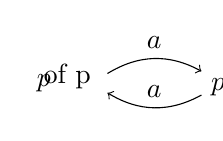
\begin{tikzpicture}
      \node (p) {$p$};
      \node[right=+40pt of p] (p') {$p'$};

      \path[->]
      (p) edge [bend left] node[above] {$a$}  (p')
      (p') edge [bend left] node[above] {$\co{a}$}  (p);
    \end{tikzpicture}
    &
    \begin{tabular}{l@{\hskip 4pt}c@{\hskip 0pt}l}
      \begin{tikzcd}
      p \arrow[r, "\co{\aa}"]
      &
      p' \arrow[d, "\aa"]
      \\
      &
      q
    \end{tikzcd}
    &$\Rightarrow$&\,\,
    $p \st{ \tau } q$ or $p = q$

    \end{tabular}
    \\[5pt]
    \boom
&

    \fwdfeedback
  \end{tabular}
  \end{equation}

The~\boom axiom states a kind of input-enabledness property,
which is however more specific as it
stipulates that the target
state of the input should loop back to the source state via a
complementary output. This is the essence of the behaviour of a
forwarder, whose role is simply to pass on a message and then get
back to its original state.
The~\fwdfeedback axiom is a weak form of Selinger's~\outputfeedback
axiom, which is better understood in conjunction with the~\boom
axiom: if the sequence of transitions $p\st{\out{a}} p'\st{a}q$ in
the~\fwdfeedback axiom is taken to be the sequence of transitions
$p'\st{\out{a}} p\st{a}p'$ in the~\boom axiom, then we see that it
must be $q=p$ in the~\fwdfeedback axiom.  Moreover, no~$\tau$ action is issued when moving from $p$ to $q$, since no
synchronisation occurs in this case: the message is just passed on.


We mechanise all this via the typeclass
\lstinline!LtsObaFW!. The overall structure of our typeclasses to reason on LTSs is thus
  $\text{\lstinline!Lts!} \geq \text{\lstinline!LtsEq!} \geq \text{\lstinline!LtsOba!}$ and
  $\text{\lstinline!LtsOba!}$ is a super-class of both \lstinline!LtsObaFB! and \lstinline!LtsObaFW!.
%% \begin{center}
%%   \scalebox{.9}{%
%%     \begin{tikzpicture}
%%       \node (Lts) {\lstinline!Lts!};
%%       \node (LtsEq) [right =+7pt of Lts]  {\lstinline!LtsEq!};
%%       \node (LtsOba) [right =+7pt of LtsEq]  {\lstinline!LtsOba!};
%%       \node (LtsFb) [above right=+7pt and +1pt of LtsOba]  {\lstinline!LtsObaFb!};
%%       \node (LtsFw) [below right=+7pt and +1pt of LtsOba]  {\lstinline!LtsObaFw!};
%%       \path[->]
%%       (Lts) edge (LtsEq)
%%       (LtsEq) edge (LtsOba)
%%       (LtsOba) edge (LtsFb)
%%       (LtsOba) edge (LtsFw);
%%     \end{tikzpicture}
%%   }
%% \end{center}
%which %
%we show in \rfig{structure-typeclasses-lts},
%along with the overall structure of our typeclasses to reason on LTSs.
We defer the details to \rapp{coq}.


To prove that~$\asleq$ is sound and complete with respect to~$\testleqS$:
\begin{enumerate} \item we define an operation to lift any LTS~$\genlts \in \obaFB$
into a suitable LTS~$\genlts_{\fw} \in \obaFW$, and \item we check the
predicates~$\cnvalong$ and~$\accP{-}{-}{-}$ over the LTS~$\genlts_{\fw}$.
\end{enumerate}
%\begin{figure}



Let~$\MO$ denote the set of all finite multisets of output actions, 
for instance we have $\varnothing, \mset{ \co{ a } }, \mset{ \co{ a },   \co{
    a }  }, \mset{ \co{ a },  \co{ b },  \co{ a },  \co{ b }} \in
\MO$.
%Similarly, let $\MI$ denote the set of all finite multisets of names.
%\ilacom{Why are the elements of $\MI$  required to be finite while those of $\MO$ are not?}
We let %$\I, \J, \ldots$ range over $\MI$ and
$M, N, \ldots$ range over~$\MO$. The symbol~$M$ stands for {\em mailbox}.
We denote with~$\uplus$ the multiset union.
We assume a function $\outputmultisetSym : A \rightarrow MO$ defined for any
LTS $\genlts_A$ of output-buffered agents such that
\begin{enumerate}[(i)]
\item
  $\co{\aa} \in O(\server)$ if and only if $\co{\aa} \in \outputmultiset{\server}$, and
\item
  for every $\server'$, if $\server \st{\co{\aa}} \server'$ then $\outputmultiset{\server} = \mset{\co{\aa}} \uplus \outputmultiset{\server'}$.
\end{enumerate}
Note that by definition $\outputmultiset{ \server }$ is a finite multiset.

\begin{definition}
  \label{def:sta}
  \label{def:liftFW}\coqLTS{lts_a}
  Let $\liftFW{\genlts} = \lts{\States \times \MO}{L}{\sta{}}$ for every LTS $\genlts = \lts{\States}{L}{\st{}}$,
%  For every LTS $\genlts = \lts{\States}{L}{\st{}}$
%  we let
%$$
%\liftFW{\genlts} = \lts{\States \times \FinMultiset{L}}{L}{\sta{}}
%$$
where the states in $\liftFW{\genlts}$ are pairs denoted $p
\triangleright \mailbox{M}$, such that $p \in \States$ and $M \in \MO$,
%is a finite multiset of outputs,
and the transition relation~$\sta{}$ is defined via the rules in
\rfig{rules-liftFW}.\hfill$\blacksquare$
\end{definition}

  



\begin{figure}
\hrulefill
  $$
  \begin{array}{llll}
    \begin{prooftree}
      \server \st{\alpha} \server'
      \justifies
      \server \triangleright M \sta{\alpha} \server' \triangleright M
    \end{prooftree}
  &
  \begin{prooftree}
    \server \st{a} \server'
    \justifies
    \server \triangleright (\mset{\co{a}} \uplus M) \sta{\tau} \server' \triangleright M
  \end{prooftree}
  \\[2em]
  \begin{prooftree}
    \justifies
    \server \triangleright (\mset{\co{a}} \uplus M) \sta{\co{a}} \server \triangleright M
  \end{prooftree}
  &
  \begin{prooftree}
    \justifies
    \server \triangleright M \sta{a} \server  \triangleright (\mset{\co{a}} \uplus M)
  \end{prooftree}
  &&
  \end{array}
  $$
  \caption{Lifting of a transition relation to transitions of forwarders.}
  \label{fig:rules-liftFW}
  \hrulefill
\end{figure}


\begin{example}
  \label{ex:forwarders-in-TACCS}
  If a calculus is fixed, then the function~$\liftFWSym$ may have a
  simpler definition.  For instance Castellani and
    Hennessy~\cite{DBLP:conf/fsttcs/CastellaniH98} define it in their
  calculus~\textsf{TACCS} by letting $\sta{\alpha}$ be the least
  relation over~\textsf{TACCS} such that
  %\item\label{pt:sta-inclusion}
  (1) for every $\alpha\in\Acttau \wehavethat \st{\alpha} {} \subseteq {} \sta{\alpha}$, and 
  %\item\label{pt:sta-asynch-input} 
  (2) for every $\aa \in \Names \wehavethat p \sta{\aa} p \Par \out{\aa}$.\hfill$\qed$
\end{example}



%%%%%%%%%%%%%%%%%%%%%%%%%%%%%%%%%%%%%%%%%%%%%%%%%%%%%%%%%%%%%
%%%%%%%%%%%%%%%%%%%%%%%%%%%%%%%%%%%%%%%%%%%%%%%%%%%%%%%%%%%%%
%%% THIS IS FOR THE THESIS
%%%%%%%%%%%%%%%%%%%%%%%%%%%%%%%%%%%%%%%%%%%%%%%%%%%%%%%%%%%%%
%%%%%%%%%%%%%%%%%%%%%%%%%%%%%%%%%%%%%%%%%%%%%%%%%%%%%%%%%%%%%
\leaveout{
NOTE. In this paragraph I explain the issues raised by defining the lifting $\genlts_\fw$
of an LTS $\genlts$ by its composition with the LTS $\Fwd_L = \lts{\MO}{L}{\st{}_{\mathit{mb}}}$
where
  \[
    M \uplus \{ \bar a \} \st{\co{a}} M
    \qquad\text{and}\qquad
    M \st{a} M \uplus \{ \bar a \}
  \]

From now, we assume that $\genlts_\fw = \genlts \times \Fwd_L$.
I will illustrate the issue using $\genlts = \lts{\ACCS}{\st{}}{\Acttau}$.

The keypoint behind the issue lies in the following question: should we consider
that $\co{a} \triangleright \varnothing \equiv 0 \triangleright \mset{\co{a}}$ ?

Let us first consider the case in which this equation is true.
First, observe that $0 \triangleright \mset{\co{a}} \stable$, which does not hold
for $\co{a} \triangleright \varnothing$ as
we can exhibit the following transition due to an interaction between $\co{a}$ and $\varnothing$.
$$
\begin{prooftree}
  \co{a} \st{\co{a}} 0 \hspace{1em} \varnothing \st{a}_{\mathit{mb}} \mset{\co{a}}
  \justifies
  \co{a} \triangleright \varnothing \sta{\tau} 0 \triangleright \mset{\co{a}}
\end{prooftree}
$$

From these two facts we have a counter example to \rlem{harmony-sta} as
$\co{a} \triangleright \varnothing \equiv 0 \triangleright \mset{\co{a}}$, and
$\co{a} \triangleright \varnothing \sta{\tau}$, but $0 \triangleright \mset{\co{a}} \stable$.
More generally, we have that the equivalence relation does not preserve stability.

We now consider the case in which this equation is false.
The output-commutativity axiom states that if
$\server \sta{\co{a}} \server_1$ and
$\server \sta{\co{a}} \server_2$ then $\server_1 = \server_2$.
We recall that in, our settings, we reason up-to equivalence between states, and thus
it should be the case that $\server_1 \equiv \server_2$.

Note that $\co{a} \triangleright \mset{\co{a}} \sta{\co{a}} 0 \triangleright \mset{\co{a}}$
and $\co{a} \triangleright \mset{\co{a}} \sta{\co{a}} \co{a} \triangleright \varnothing$.
However, by considering $\co{a} \triangleright \varnothing \nequiv 0 \triangleright \mset{\co{a}}$
we have that $\genlts_\fw$ does not obey to the output-commutativity axiom.
}
%%%%%%%%%%%%%%%%%%%%%%%%%%%%%%%%%%%%%%%%%%%%%%%%%%%%%%%%%
%%%%% END OF LEAVEOUT
%%%%%%%%%%%%%%%%%%%%%%%%%%%%%%%%%%%%%%%%%%%%%%%%%%%%%%%%%
%% \leo{%                                                                           %%
%%   to work with LTSs we define the lifting in a more abstract manner, by          %%
%%   composition with an LTS~$\Fwd_L =                                              %%
%%   \lts{\FinMultiset{L}}{L}{\st{}_{\mathit{mb}}}$ of mailboxes, whose states      %%
%%   are finite multisets~$M$ of messages, and with two types of transitions:       %%
%%   %                                                                              %%
%%   \[                                                                             %%
%%     M \uplus \{ \bar a \} \st{\co{a}} M                                          %%
%%     \qquad\text{and}\qquad                                                       %%
%%     M \st{a} M \uplus \{ \bar a \}                                               %%
%%   \]                                                                             %%
%%   %                                                                              %%
%%   The lifting~$\genlts_\fw$ of an LTS $\genlts = \lts{\States}{L}{\st{}}$ is     %%
%%   then defined as the product LTS: $\genlts \times \Fwd_L$, whose states are     %%
%%   pairs which we write $p \triangleright \mailbox{M}$ where $p \in \genlts$ is a %%
%%   server, and $M$ is a finite multiset of outputs.                               %%
%% }                                                                                %%

The transition relation $\sta{}$ is reminiscent of the one introduced
in Definition 8 by Honda and
  Tokoro in~\cite{DBLP:conf/ecoop/HondaT91}.  The construction given in
our \rdef{liftFW}, though, does not yield the LTS of Honda and Tokoro,
as $\sta{}$ adds the forwarding capabilities to the states only at the
top-level, instead of descending structurally into terms. As a
consequence, in the LTS of~\cite{DBLP:conf/ecoop/HondaT91}
$\aa.\Nil + \Nil \st{ \ab } \co{ \ab }$, while
$\aa.\Nil + \Nil \Nsta{ \ab } \co{ \ab }$.


\begin{example}
  As the set~$\Names$ is countable, every process~$\server$ in
  the LTS $\lts{\ACCS \times \MO}{\Acttau}{\sta{}}$ is
  infinitely-branching, %
  for instance for every $\server$ and every input $\mu$ we have %
    $ \server \st{\mu} \server \Par \co{\mu}$, %
    hence $\server \st{\aa_0} \server \Par \co{\aa_0}$,
    $\server \st{\aa_1} \server \Par \co{\aa_1}$,
    $\server \st{\aa_2} \server \Par \co{\aa_2}$, \ldots
  \hfill$\qed$
    %%% FOR THE JOURNAL VERSION
%as illustrated in the picture below,
%%    where we show only the part of the LTS that is added
%%    by the lifting to $\sta{}$.
    %% \ilacom{maybe we should
    %% say that the we show only the part of the LTS that is added
    %% by the lifting to $\sta{}$.}
%% \begin{center}
%%   \scalebox{.7}{%
%%   \begin{tikzpicture}
%%   \node[state](t){$\server \triangleright \varnothing$};

%%   \node[state][below=  of t](p20){$\server \triangleright \mailbox{\co{\aa_2}}$};
%%   \node[state][below=  of p20] (nil){$\server \triangleright \varnothing$};

%%   \node[state][left=of p20] (p10) {$\server \triangleright \mailbox{\co{\aa_1}}$};

%%   \node[state][left =of p10] (p00) {$\server \triangleright \mailbox{\co{\aa_0}}$};

%%   \node[state][right=of p20](p30){$\server \triangleright \mailbox{\co{\aa_3}}$};

%%   \node[][right=of p30](p5){\vdots\ldots\vdots};

%% %Edges
%% \path (t) edge[to] node[action,swap] {$\aa_0$} (p00)
%%       (t) edge[to] node[action] {$\aa_1$} (p10)
%%       (t) edge[to] node[action] {$\aa_2$} (p20)
%%       (t) edge[to] node[action,yshift=-8pt] {$\aa_3$} (p30)
%%       (t) edge[to] node[action] {$\aa_4$} (p5);

%% \path
%% (p00)  edge[to] node[action, swap] {$\co{\aa}_0$} (nil)
%% (p10)  edge[to] node[action] {$\co{\aa}_1$} (nil)
%% (p20)  edge[to] node[action] {$\co{\aa}_2$} (nil)
%% (p30)  edge[to] node[action, right] {$\co{\aa}_3$} (nil)
%% (p5)  edge[to] node[action] {$\co{\aa}_4$} (nil);
%%   \end{tikzpicture}
%%   }
%% \end{center}
    %% \vspace{-12pt}
\end{example}

%\gb{TODO ILARIA, check and possibly improve the explanation ?}
The intuition behind \rdef{sta} %\rdefpt{sta}{sta-asynch-input} \ilacom{I see no point $(ii)$ in this definition}
is that, when a client interacts with a server asynchronously, the
client can send any message it likes, regardless of the inputs that
the server can actually perform. In fact, asynchronous clients behave
as if the server was saturated with \emph{forwarders}, namely
processes of the form $\aa. \co{\aa}$, for any $\aa\in\Names$.


\noindent
We are ready to state two main properties of the
function~$\liftFWSym$: it lifts any LTS of output-buffered agents with feedback
to an LTS of forwarders, and the lifting preserves the~$\opMust$ predicate. We can therefore
reason on~$\testleqS$ using LTSs of forwarders.% (\rcor{testleq-obafb-iff-testleq-obafw}).

\begin{lemma}
  \label{lem:liftFW-works}
  For every LTS~$\genlts \in \obaFB$, $\liftFW{\genlts} \in \obaFW$.
\end{lemma}
%% \begin{proof}
%%   \TODO{Paul, WRITE ME}
%% \end{proof}


\begin{lemma}
  \label{lem:musti-obafb-iff-musti-obafw}
  For every $\genlts_A, \genlts_B, \genlts_C \in \obaFB, \serverA \in A, \serverB \in B, \client \in C$,
  \begin{enumerate}
    \item
      $\musti{\server}{\client}$ if and only if $\musti{\liftFW{\server}}{\client}$,
    \item
      $\serverA \testleqS \serverB$ if and only if $\liftFW{\serverA} \testleqS \liftFW{\serverB}$.
  \end{enumerate}
\end{lemma}

%% \begin{corollary}
%%   \label{cor:testleq-obafb-iff-testleq-obafw}
%%   For every $\genlts_A, \genlts_B  \in \obaFB, \serverA \in A, \serverB \in B$,
%%   $\serverA \testleqS \serverB$ if and only if $\liftFW{\serverA} \testleqS \liftFW{\serverB}$.
%% \end{corollary}


%\TODO{Why are ObaFW useful if must is logically equivalent to obaFB?}


%%%%%%%%%%%%%%%%% DEFINITION ABSTRACTION FOR ALTERNATIVE PREORDER
%% USELESS
%% Surprisingly, two predicates suffice to define our first alternative
%% preoder.  First, we define convergence along traces on the LTS of
%% Honda and Tokoro, \ie the predicate~$\acnvalong$, exactly
%% as~$\cnvalong$ but based on the transition relation~$\sta{}$.

%% The second abstraction that we need is an asynchronous variant
%% of the {\em acceptance sets}
%% of~\cite{DBLP:journals/jacm/Hennessy85}:%
%% (\coqMT{acceptance_sets}):

%% NOW USELESS
%We define weak transitions~$\wta{s}$~in the standard inductive way,% (\coqLTS{weak_a}),
%\ie via the same rules used to define~$\wt{s}$.
We now simplify the definition of acceptance sets to reason on
forwarders: %LTSs that are \obaFW:
for any two LTS $\genlts_\StatesA, \genlts_\StatesB \in \obaFW$ and servers
$ \serverA \in \StatesA$, and $\serverB \in \StatesB$  we let
$\accfwp{ \state }{ \trace }{ \st{} } =  \setof{ O(\state') }{ \state
  \wt{ \trace } \state' \stable }$.
This definition suffices to characterise~$\testleqS$ because in each LTS that is \obaFW\ every state performs
every input, thus comparing inputs has no impact on the
preorder~$\bhvleqtwo$ of \rdef{standard-char}. More formally,
for every $\genlts_\StatesA, \genlts_\StatesB \in \obaFW$ and every $\server \in \StatesA$ and $\serverB \in \StatesB$,
we let %$\serverA \asleqAfw \serverB \text{ iff } \text{ iff }$
$$
\serverA \asleqAfw \serverB \text{ iff } \forall \trace \in \Actfin \wehavethat \serverA \cnvalong \trace \implies \accfwp{ \serverA }{ \trace }{ \st{}_\StatesA } \ll \accfwp{ \serverB }{ \trace }{ \st{}_\StatesB }
$$
Then we have the following logical equivalence.
\begin{lemma}
  \label{lem:conditions-on-accsets-logically-equivalent}
  Let $\genlts_A, \genlts_B \in \obaFW$.
  For every $\serverA \in \StatesA, \serverB \in \StatesB, \serverA \bhvleqtwo \serverB$
  if and only if $\serverA \asleqAfw \serverB$.
\end{lemma}
\begin{proof}
  The {\em only if} implication is trivial, so we discuss the {\em if}
  one. Suppose that $ \serverA \asleqAfw \serverB  $ and that for some
  $\trace$ we have that $R \in \accP{\serverB}{s}{\st{}_B}$. Let~$X$ be
  the possibly empty subset of~$R$ that contains only output actions.
  Note that since~$\genlts_B$ is~\obaFW\ we know by definition that $R =
  X \cup \Names$.
  By definition $X \in \accfwp{\serverB}{s}{\st{}_B}$, and thus by
  hypothesis there exists some set of output actions $Y \in
  \accfwp{\serverA}{s}{\st{}_A}$ such that $Y \subseteq X$.
  It follows that the set $Y \cup \Names \in
  \accP{\serverA}{s}{\st{}_A}$, and trivially $Y \cup \Names \subseteq
  X \cup \Names = R$.
\end{proof}


  %%%%%%%%%
  %%%%%%%%%
  %%%%%%%%% END OF \gb



%%% ACCEPTANCE SETS EXPLAINED EARLIER FOR THE STANDARD ALTERNATIVE
%%% CHAR BY MATTHEW
%% If~$O( \server ) = \emptyset$ then~$\server$ can only wait for an
%% output sent by the client. Acceptance sets then capture, in spite of
%% \nondeterminismT, all the outputs that potential deadlock states in
%% the server offer to the environment (\ie the client).

%%% ARE THESE NEEDED ?
\renewcommand{\serverA}{p}
\renewcommand{\serverB}{q}

%% We are now ready to define our first characterisation.
%% \begin{definition}[Behavioural preorder]%\coqMT{bhv_pre}]
%%   \label{def:bhv-leq}%
%%   We write $ \serverA \bhvleq \serverB $ whenever
%%   $\serverB \bhvleqone
%%   \serverA  \wedge  \serverA \asleqAfw \serverB$.\hfill$\blacksquare$
%% \end{definition}


In view of the second point of \rlem{musti-obafb-iff-musti-obafw},
to prove completeness it suffices to show that~$\asleq$
includes~$\testleqS$ in the LTS of
forwarders. This is indeed true:
\begin{lemma}
  \label{lem:completenessA}
  For every $\genlts_A, \genlts_B \in \obaFW$ and
  servers $\serverA \in \StatesA, \serverB \in \StatesB $,
  if ${ \serverA } \testleqS { \serverB }$
  then ${ \serverA } \asleq { \serverB }$.
\end{lemma}


%{\em Notation:}
%To simplify the statements of our theorems we slightly abuse the
%notation.
%With a slight
By a slight abuse of notation,
given an LTS $\genlts = \lts{\States}{L}{\st{}}$ and a state
$\server \in \States$,
we denote with $\liftFW{
  \server }$ the LTS rooted at $\server \triangleright \mailbox{ \emptyMset }$ in $\liftFW{\genlts}$.


\begin{theorem}%% \coqEq{ctx_iff_bhv} %%
  \label{thm:testleqS-equals-bhvleq}
  \label{thm:testleqS-equals-accleq}
  \label{thm:testleqS-equals-asleq}
  For every $\genlts_A, \genlts_B \in \obaFB$
  and $\serverA \in \States, \serverB \in \StatesB, \,
  \serverA \testleqS \serverB$ if and only if
  $\liftFW{\serverA} \asleq \liftFW{\serverB}$.
\end{theorem}
%% \begin{proof}
%%   We discuss the steps of the proof
%%   in \rsec{bhv-completeness}-\ref{sec:bhv-soundness}.
%% \end{proof}

The proof of completeness is given in \rapp{proof-completeness},
where the main aim is to show \rlem{completenessA}.
The proof of soundness, instead, requires much more
auxiliary machinery than the one used to state \rlem{completenessA},
so we defer it entirely to \rapp{proof-soundness}.
Here we highlight the major novelty with respect to the literature, via a little digression.
All the soundness arguments for behavioural characterisations of
$\testleqS$ in non-deterministic settings,
for instance~\cite{DBLP:journals/tcs/NicolaH84,DBLP:journals/jlp/Hennessy05,DBLP:journals/fac/HennessyI93,DBLP:journals/iandc/BorealeN95,DBLP:journals/corr/BernardiH15}
but to cite a few, are rooted in classical logic, because they
(1) unzip %potentially infinite
maximal computations of 
$\csys{ \server }{ \client }\st{}\cdots$  %(which cannot be done
%constructively)
to produce traces $ \server \wt{ \trace } $ and $ \client
\wt{ \co{ \trace } } $ that may be infinite;
%%  \item\label{pt:excluded-middle}
(2) use the excluded middle on an undecidable property,
namely the infinity of the traces at hand; and 
%\item\label{pt:koenigs}
(3) in case of infinite traces apply \koenigslemma
(see for instance lemmas 4.4.12 and 4.4.13 of~\cite{DBLP:books/daglib/0066919}).
Our proof replaces \koenigslemma with induction and works
on infinite branching STS. This is possible thanks to the \barinduction\ principle,
which we outline in \rsec{barinduction-main-body}.

% An immediate consequence of~\rlem{ACCS-obaFB} and
% ~\rthm{testleqS-equals-accleq} is a characterisation of~$\testleqS$
% for~$\ACCS$:

From~\rlem{ACCS-obaFB} and~\rthm{testleqS-equals-accleq} we
immediately get a characterisation of~$\testleqS$ for~$\ACCS$:
\begin{corollary}
  \label{cor:characterisation-for-aCCS}
For every $\serverA, \serverB \in \modulo{\ACCS}{\equiv}, \serverA \testleqS \serverB$ if and only if $\liftFW{\serverA} \asleq
\liftFW{\serverB}.$
\end{corollary}

In \rapp{normal-form} we present what, to the best of our knowledge,
are the first behavioural characterisations of the \mustpreorder that
fully exploit asynchrony, \ie disregard irrelevant (that is, non-causal)
orders of visible actions in traces. Due to space constraints, here
we omit these additional results.

%This is possible thanks to the \outputcommutativity axiom.
%, and an analogous property for inputs that forwarders enjoy.
%%%% NO LONGER USEFULL
%% These alternative preorders use finite sequences of (pairs of)
%% multisets of inputs and multisets of outputs \ie sequences $
%% (\I_1,M_1) \ldots (\I_n,M_n)$, instead of standard sequences of actions.




\newcommand{\msleqtwo}{\preccurlyeq_{\textsc{m}}}

\subsection{The \MustSet approach}
As first application of \rthm{testleqS-equals-asleq}, we prove that the
second standard way to characterise the preorder~$\testleqS$, \ie
the one based on \MustSets, is indeed sound and complete.

\renewcommand{\after}[3]{ (#1 \, \mathsf{after} \,  #2, #3) }

For every~$X \subseteq_{\mathit{fin}} \Act$, that is for every finite set of visible actions,
with a slightly abuse of notation we write $\server \mathrel{\opMust} X$ whenever $\server \wt{ \varepsilon } \server'$ implies that $\server' \st{ \mu }$ for some $\mu \in X$, and we say that~$X$ is a \MustSet of~$\server$.
Let $\after{ \serverA }{ s }{ \st{} } = \setof{ \serverA' }{ \serverA \wt{s} \serverA' }$.
For every $\genlts_\StatesA, \genlts_\StatesB$ and $\serverA \in \StatesA, \serverB \in \StatesB$,
let $\serverA \msleqtwo \serverB$ whenever
$\forall \trace \in \Actfin$ we have that $\serverA \cnvalong{ \trace
}$ implies that $(\forall X \subseteq_{\mathit{fin}} \Act$ if
$\after{\serverA}{\trace}{ \st{}_\StatesA } \mathrel{\opMust} X$ then
$\after{\serverB}{\trace}{ \st{}_\StatesB } \mathrel{\opMust} X).$



\begin{definition}
  \label{def:denicola-char}
  For every $\genlts_A, \genlts_B \in \obaFB$, and server $\serverA
  \in A$ and $\serverB \in B$ we let $\serverA \msleq \serverB$ whenever
  $\serverA \bhvleqone \serverB \wedge
  \serverA \msleqtwo \serverB$.\hfill$\blacksquare$
\end{definition}


\begin{lemma}
  \label{lem:acceptance-sets-and-must-sets-have-same-expressivity}
  Let $\genlts_A, \genlts_B \in \obaFB$.
  For every $\serverA \in \StatesA, \serverB \in \StatesB $ such that $\liftFW{\serverA} \bhvleqone \liftFW{\serverB}$,
  we have that
  $\liftFW{\serverA} \msleqtwo \liftFW{\serverB}$ if and only if
  $\liftFW{\serverA} \asleqAfw \liftFW{\serverB}$.
\end{lemma}
\noindent
As a direct consequence, we obtain our second result.
\begin{theorem}
  \label{thm:testleqS-equals-mustsetleq}
    Let $\genlts_A, \genlts_B \in \obaFB$.
  For every $\serverA \in \States$  and
  $\serverB \in \StatesB $, we have that
  $\serverA \testleqS \serverB$ if and only if
  $\liftFW{\serverA} \msleq \liftFW{\serverB}$.
\end{theorem}
%% \begin{proof}
%%   It suffices to prove that $ \serverA \preccurlyeq_{\textsc{ms}} \serverB $ if and only if
%%   $ \serverA \preccurlyeq_{\textsc{m}} \serverB $. This is \rlem{acceptance-sets-and-must-sets-have-same-expressivity}.
%% \end{proof}


\newcommand{\failleq}{\mathrel{\leq_{\textsf{fail}}}}

{\bfseries Failure refinement.} %
\MustSets\ have been used mainly
by De Nicola and collaborators, for instance
in~\cite{DBLP:journals/lmcs/NicolaM23,DBLP:journals/iandc/BorealeNP02},
and are closely related to the failure refinement proposed
in~\cite{DBLP:journals/jacm/BrookesHR84} by Hoare, Brookes and Roscoe for TCSP (the process
algebra based on Hoare's language CSP
\cite{DBLP:journals/cacm/Hoare83a,DBLP:conf/icalp/Brookes83}).
Following~\cite{DBLP:journals/jacm/BrookesHR84},  
a {\em failure} of a process $\server$ is a pair $(\trace, X)$
such that $p \wt{ \trace } p'$ and $p' \Nst{\mu}$ for all $\mu \in X$.
Then, failure refinement is defined by letting $\serverA\failleq\serverB$
whenever the failures of~$\serverB$ are also failures of $\serverA$.
%This refinement is the staple of the community focused on 
%its variants have been applied to
%verify the software in the Russian module of the International Space Station 
%\cite{DBLP:conf/birthday/PeleskaB99,DBLP:conf/amast/ButhKPS97,DBLP:conf/amast/ButhPS98},
%Practitioners using failure refinements rely on the tool FDR
%\cite{DBLP:journals/sttt/Gibson-Robinson16}, and a number of
This refinement was designed to give a denotational semantics to
processes, and mechanisations in Isabelle/HOL have been
developed to ensure that the refinement
is well defined~\cite{HOL-CSP-AFP,DBLP:journals/acta/BaxterRC22}.  Both
Hennessy~\cite[pag. 260]{DBLP:books/daglib/0066919}
and~\cite{Castellan2023}
% \cite{DBLP:journals/corr/abs-2108-10558}
highlight that the failure
  model can be justified operationally via the~$\opMust$ testing
  equivalence: it is folklore dating back to~\cite[Section
    4]{DBLP:journals/tcs/NicolaH84} that failure equivalence and~$\testeq$ coincide.
  Thanks to \rthm{testleqS-equals-mustsetleq} we
  conclude that in fact~$\testleqS$ 
  coincides with~$\failleq$ in conjunction with~$\bhvleqone$.\footnote{The preorder becomes 
  then the ``failure divergence'' refinement formalised as
  $\sqsubseteq_{\text{\tt FD}}$ in \url{https://www.isa-afp.org/sessions/hol-csp/\#Process\_Order.html}.}
%%\ilacom{Check that this has not be proven before.}

  
\begin{corollary}
  \label{cor:testleqS-equals-failleq}
  Let $\genlts_A, \genlts_B \in \obaFB$.
  For every $\serverA \in \States$  and
  $\serverB \in \StatesB $, we have that
  $\serverA \testleqS \serverB$ if and only if
  $\liftFW{\serverA} \bhvleqone \liftFW{\serverB}$
  and $\liftFW{\serverA} \failleq \liftFW{\serverB}$.
\end{corollary}
%% \begin{proof}
%%   Suppose that $\serverB$ refuses $(s,X)$, then
%%   $\lnot (\serverB \mathrel{\opMust} (s,X))$,
%%   and thus $\lnot (\serverA \mathrel{\opMust} (s,X))$,
%%   which menas that $\serverA$ refuses $(s,W)$.
%% \end{proof}


%%% FOR LONG VERSION
%% {\bfseries Further applications.}
%% Thanks to our alternative preorders, 
%% we also formalise an intuition
%% that comes from our every-day experience: in an asynchronous world, a
%% server that performs only inputs is useless, \ie it can be replaced by a
%% completely inactive program, like~$\Nil$ in $\ACCS$.

%% \begin{proposition}
%%   \label{prop:only-inputs-imply-uselessness}
%%   For every $\genlts_\StatesA \in \obaFB$ and $\server \in \StatesA$,
%%   if for every $\trace \in \Actfin . \, \server \wt{\trace} \st{
%%     \alpha}$ implies that $\alpha \in \Names$ then $\server \testleqS \Nil$.
%% \end{proposition}





\section{\Barinduction: from \extensional to \intentional definitions}
\label{sec:barinduction-main-body}
Two predicates are crucial to reason on the \mustpreorder,
namely passing a test, \ie $\opMust$, and convergence, \ie $\conv$.
Both predicates are defined in an {\em \extensional} manner,
\ie by requiring that for every infinite sequence
there exists a state that is in some sense good. These are respectively the
predicate $\goodSym$ in the definition of $\opMust$ and the predicate
of stability, \ie $\Nst{}$, in the definition of convergence.

Both \extensional predicates can actually be defined inductively,
following an {\em \intentional} approach.
Let $\mathsf{int}_Q$ be the inductive predicate (least
fixpoint) defined by the following rules:
  $$
  \begin{array}{l@{\hskip 2pt}l@{\hskip 20pt}l@{\hskip 2pt}l}
    \rname{axiom}
&    \begin{prooftree}
      Q(s)
      \justifies
      \mathsf{int}_Q(s)
    \end{prooftree}
    &
    \rname{ind-rule}
    &
    \begin{prooftree}
      s \to
      \qquad
      \forall s' \wehavethat  s \to s' \implies \mathsf{int}_Q(s')
      \justifies
      \mathsf{int}_Q(s)
    \end{prooftree}
  \end{array}
  $$
and we define our inductive predicates via $\mathsf{int}$ by letting
$\state \convi \eqdef  \mathsf{int}_{Q_1}( \state )$
and $\musti{ \server }{\client } \eqdef \mathsf{int}_{Q_2}(\state, \client )$,
where $Q_1(\state) \eqdef \state \Nst{\phantom{\tau}}$ and  %\qquad\qquad
$Q_2(\state, \client) \eqdef \good{\client}$.


While proving that the \intentional predicates ($\opMusti$ and~$\convi$)
imply the \extensional ones ($\opMust$ and~$\conv$) are easy arguments by
induction, proving the converse implications is a known problem.
Its constructive solution rests on either the fan-theorem or the
\barinduction principle. The first applies to finite branching trees,
while the second to countably infinite branching trees. We favour
\barinduction because in calculi like infinitary CCS computations
can form countably branching trees.

\begin{proposition}%% \coqBar{extensional_implies_inductive} %%
  Given a countably branching STS~$\sts{\SysStates}{\to}$, and a decidable predicate~$Q$
  on~$\SysStates$, for all~$s \in \SysStates$, $\mathsf{ext}_Q(s)$ implies
  $\mathsf{int}_Q(s).$
\end{proposition}

\begin{corollary}
  \label{cor:ext-int-eq-conv}
  \label{cor:ext-int-eq-must}
  For every $\server \in \States$,
%  \begin{enumerate}
  % \item
  (1) $\state \conv $ if and only if $\state \convi$,
%\item
  (2) for every $\client$ we have that $\Must{\server}{\client}$ if
    and only if $\musti{\server}{\client}$.
%  \end{enumerate}
\end{corollary}
\noindent

Thanks to this corollary, in the proofs of the characterisations of~$\testleqS$,
and in our code, we use the predicates~$\opMusti$ and~$\convi$. In other terms,
we reason by induction.

The details about \barinduction, our mechanisation,
and the proofs of the above results are deferred to \rapp{bar-induction}.


%% \begin{lemma}[\coqMT{weak_a_congr_up_to_permutation}]
%%     \label{lem:weaka-congr-switch-s}
%%     \label{lem:wta-preserved-by-permutation-inputs}
%%   For every $p, q$, and
%%   $s, t \in \Names^\star \wehavethat \perm{s}{t}$ and $p \wta{s} q$ imply $p \wta{t} \cdot \equiv q$.
%% \end{lemma}
%% \noindent
%% where $\perm{s}{t}$ means that $s$ is a permutation of $t$. An easy consequence is that
%% %\rlem{weak-a-swap} implies that
%% convergence is preserved by permuting inputs:

%% \begin{lemma}[\coqMT{acnv_up_to_permutation}]%{mylemma}{existsacnvaimpliesforallacnvaperm}
%%   \label{lem:exists-acnva-implies-forall-acnva-perm}
%%   $\Forevery p \in \Proc \and s,t \in \Names^\star \wehavethat \perm{s}{t}$ and
%%   $p \acnvalong{s} \imply p \acnvalong{t}$.
%% \end{lemma}

%% If we consider also infinite multisets $\I$
%% in \rdefptNOPAR{ff-good}{ff4-acc-sets},
%% then the preorder is not complete. We discuss this in
%% \rexa{finite-multisets-necessary}.

%% In the next two examples we prove that
%% both conditions of \rdef{ff-good} are necessary to prove the soudness of $\testleqS$.

%% \begin{example}
%%         \gb{Show that \rpt{ff4-conv} of \rdef{ff-good} is complete but not sound.}\hfill$\qed$
%% \end{example}


%% \begin{example}
%%         \gb{Show that \rpt{ff4-acc-sets} of \rdef{ff-good} is complete but not sound.}\hfill$\qed$
%% \end{example}



%% We have alredy seen in \rlem{standard-property} does not hold for input actions in the
%% asynchronous CCS, because \rptlem{standard-property}{standard-property-1} is false.
%% The situation does not improve much in
%% the LTS $\sta{}$, because even though the analogous of \rptlem{standard-property}{standard-property-1} is true,
%% it is the analogous of \rptlem{standard-property}{standard-property-2} that is false.



%% \begin{restatable}[COQ LINK]{mylemma}{testleqSpreservedbyrightactioninput}
%%   \label{lem:testleqS-preserved-by-right-action-input}
%%   For every $p,q$, $\mu \in \Names$,
%%   if $p \testleqS q$ and $q \wt{\mu} q'$
%%   then there exists $p'$ such that
%%   $p \wta{\mu} p'$ and $p' \testleqS q'$.
%% \end{restatable}
%% \begin{proof}
%% \gb{We decompose the reduction $q \wta{\mu} q'$ as follows:
%%   $$
%%   q \wta{\varepsilon} q_0 \st{\mu} q_1 \wta{\varepsilon} q'
%%   $$
%%   \rcor{testleqS-included-by-right-tau} and the transitivity of the preorder
%%   ensure that $q \testleqS q_0$ and $q_1 \testleqS q'$.
%%   The hypothesis imply  $p \testleqS q_0$, and that it
%%   it suffices to prove $p' \testleqS q_1$, for some $p'$
%%   such that $p \wt{\mu} p'$.

%%   If $\mu$ is an input we use \rdefpt{sta}{sta-asynch-input} to prove $p \wta{\mu} p \Par \mailbox{\co{\mu}}$.
%%   We prove $p \Par \mailbox{\co{\mu}} \testleqS q_1$.
%%   Now let $p \Par \mailbox{\co{\mu}} \musti r$ for some $r$.
%%   If $r \st{\ok}$ then trivially $q_1 \musti r$. If $r$ is unsuccesful,
%%   then we apply \rlem{must-i-output-swap} to show that $p  \musti r \Par \mailbox{\co{\mu}}$,
%%   and thus $ q_0 \musti r \Par \mailbox{\co{\mu}} $. The transition $ q_0 \st{\mu} q_1$ and
%%   \rlem{musti-presereved-by-actions-of-unsuccesful-tests} imply $ q_1 \musti r $.


%%   If $\mu$ is an output, then observe that $q \Nmusti \co{\mu}.\Nil \extc \tau.\Unit$,
%%   thus by hypothesis $p \Nmusti \co{\mu}.\Nil \extc \tau.\Unit$, and we obtain $p \wta{\mu} p'$
%%   via \rlem{action-or-pass}. \rlem{output-shape} implies $ p \equiv p' \Par \mu $
%%   and that $q \equiv q' \Par \mu$. We conclude via \rlem{testleqS-output-annhil}.}
%%   %% Thanks to \rdefpt{sta}{sta-asynch-input} we know that
%%   %% $p \wta{\mu} p \Par \co{\mu}$.
%%   %% We must show that $p \Par \co{\mu} \testleqS q'$.
%% %% We decompose the reduction $q \wta{\mu} q'$ as follows:
%% %% $$
%% %% q \wta{\varepsilon} q_0 \st{\mu} q_1 \wta{\varepsilon} q'
%% %% $$
%% %% \rcor{testleqS-included-by-wta-epsilon} ensures that
%% %% $p \testleqS q_0$.
%% %% \rlem{must-i-output-swap} ensures that
%% %% $p \Par \co{\mu} \testleqS q_1$ (be more explicit here) and
%% %% \rcor{testleqS-included-by-wta-epsilon}
%% %% allows us to conclude that $p \Par \co{\mu} \testleqS q'$.
%% \end{proof}
%% \gb{Is the hypothesis of $\mu$ being an input necessary ?}


%% \begin{example}
%%   \label{ex:partB-of-standard-lemma-fails}
%% Take $\mu = a$, $p' = \tau.\Nil \extc c.\co{b} $ and $p = p' \Par \mailbox{\co{a} \Par \co{c}}$.
%% By reflexivity $p \testleqS p$, and by definition there exist the transitions
%% $$
%% \begin{array}{l}
%% p \st{\co{a}} \equiv p' \Par \mailbox{\co{c}}
%% \\
%% p \wta{ \co{a} } \st{\tau} \mailbox{\co{b}} \Par \Nil
%% \end{array}
%% $$
%% thus $ \mailbox{\co{b}} \in ( p \aftera \co{a} )$.
%% We have that $\co{b} \NtestleqS p' \Par \co{c}$
%% because $\co{b} \musti b.\Unit$, while the maximal computation
%% $$
%% \svr[ p' \Par \mailbox{\co{c}} ] \Par \clt[  b.\Unit ] \st{\tau}
%% \svr[ \Nil \Par \mailbox{\co{c}} ] \Par \clt[  b.\Unit ] \stable
%% $$
%% witnesses that
%% $p' \Par \mailbox{\co{c}} \Nmusti b.\Unit$. It follows that $  ( p \aftera \co{a} ) \NtestleqS q'$.\qed
%% %  It is not true that for every $p$, $q$, and $q'$, $\mu \in \Names$,
%% %  if $q \st{\co{\mu}} q'$ then for every $p'$ such that
%% %  $p \wta{\co{\mu}} p'$, then $p' \testleqS q'$.
%%   %% Take $\mu = a$,
%%   %% $p = q = (\tau.\Nil \extc \tau.\co{b}) \Par \co{a}$.
%%   %% It is clear that $p \testleqS q$, $q \st{\co{a}} (\tau.\Nil \extc \tau.\co{b}) \Par \Nil$
%%   %% and $p \wta{\co{\mu}} \co{b} \Par \Nil$, but $\co{b} \NtestleqS \tau.\Nil \extc \tau.\co{b}$
%%   %% as $\co{b} \NtestleqS \tau.\Nil \extc \tau.\co{b}$.
%%   %% As a consequence we need a more precise Lemma to catch the desired $p'$,
%%   %% as we try in \rlem{testleqS-output-inversion}.
%% \end{example}

\newcommand{\oh}{\mathcal{O}_p}
\newcommand{\ohmy}{O}
\newcommand{\ogood}{O_{\mathsf{good}}}
\renewcommand{\States}{C}


\section{Conclusion}
\label{sec:conclusion}


Hopefully there is something smart to say.


%% %%%% OLD TEXT FROM ESOP PAPER
%% In this paper we have shown that the standard characterisations of
%%   the \mustpreorder by De Nicola and
%%   Hennessy~\cite{DBLP:journals/tcs/NicolaH84,DBLP:books/daglib/0066919}
%%   are sound and complete also in an asynchronous setting, provided servers are
%%   enhanced with the forwarding ability.
%%   \rlem{liftFW-works} shows that this lifting is always possible.
%%   %
%%   We have also shown that the standard coinductive characterisation carries over to the
%%   asynchronous setting.
%%   %
%%   Our results 
%%   are supported by 
%%   the first mechanisation of the \mustpreorder, and increase proof
%%   (i.e. code) factorisation and reusability since the alternative preorders
%%   do not need to be changed when shifting between synchronous and
%%   asynchronous semantics: it is enough to parameterise the proofs on
%%   the set of non-blocking actions.
%% %
%%   \rcor{testleqS-equals-failleq} states that \mustpreorder and failure
%%   refinement essentially coincide. This might spur further interest in
%%   the mechanisations of the latter
%%   \cite{HOL-CSP-AFP,DBLP:journals/acta/BaxterRC22}, possibly leading
%%   to a joint development.%



%% \paragraph{Proof method for \mustpreorder}
%% Theorems \ref{thm:testleqS-equals-asleq}, \ref{thm:coinductive-char-equiv-main}
%% and \ref{thm:testleqS-equals-mustsetleq} endow researchers in programming
%% languages for message-passing software with a proof method for~$\testleqS$,
%% namely: to define for their calculi an LTS that enjoys the axioms of
%% output-buffered agents with feedback.
%% An example of this approach is \rcor{characterisation-for-aCCS}.


%% \paragraph{Live programs have barred trees}  We argued that a proof
%% of $\Must{\server}{\client}$ is a proof of liveness (of the
%% client). This paper is thus de facto an example that proving
%% liveness amounts to prove that a computational tree has a bar (identified
%% by the predicate $\goodSym$), and hence \barinduction is a natural way
%% to reason constructively on liveness-preserving manipulations on programs.
%% While this fact seems to be by and large 
%% unexploited by the PL community, we believe that it may 
%% be of interest to practitioners reasoning on liveness
%% properties 
%% in theorem provers in particular, and to the PL
%% community at large.

%% \paragraph{Mechanisation} %
%% Boreale and Gadducci~\cite{DBLP:journals/tcs/BorealeG06} remark that the
%% \mustpreorder lacks a tractable proof method.  In constrast, we argue that our
%% contributions, in particular the coinductive characterisation
%% (\rthm{coinductive-char-equiv-main}), being fully mechanised in Coq, let
%% practitioners pursue non-trivial results about testing preorders for real-world
%% programming languages.  
%% %
%% To make this point, we have proved a form of code-hoisting using this
%% characterisation.
%% %
%% Our mechanisation lowers the barrier to entry for
%% researchers versed into theorem provers and wishing to use testing preorders;
%% adds to the toolkit of Coq users an alternative to the well-known (and already
%% mechanised) bisimulation equivalence \cite{DBLP:conf/lics/Pous16}; and provides
%% a starting point for researchers willing to study testing preorders and
%% analogous refinements within type theory.  Our code is open-source and available
%% on-line. %Practitioners
%% Researchers working on testing preorders may benefit from it, as
%% there are analogies between reasoning techniques for \textsc{May}, $\opMust$,
%% \textsc{Compliance}, \textsc{Should}, and \textsc{Fair} testing. For instance
%% Baldan et al. show with pen and paper that a technique similar to forwarding
%% works to characterise the $\May$-preorder~\cite{DBLP:conf/birthday/BaldanBGV15}.
%% %  

%% \paragraph{Future work}  Thanks to Theorems \ref{thm:testleqS-equals-asleq},
%% \ref{thm:coinductive-char-equiv-main} and \ref{thm:testleqS-equals-mustsetleq}
%% we can now set out to (1) devise an
%% axiomatisation of~$\testleqS$ for asynchronous calculi, as done in
%% \cite{DBLP:journals/fac/HennessyI93,DBLP:journals/iandc/BorealeN95,DBLP:books/daglib/0066919,DBLP:journals/tcs/Hennessy02}
%% for synchronous ones; (2) study for which asynchronous calculi~$\testleqS$ is a
%% pre-congruence; (3) machine-check semantic models of subtyping for session types
%% \cite{DBLP:journals/mscs/BernardiH16}; (4) study the decidability
%% of~$\testleqS$.  We conjecture that in Selinger asynchronous setting the
%% \mustpreorder is undecidable.

%% More in general, given the practical relevance of asynchronous
%% communication, it seems crucial %
%% not only to adapt the large body of theory for synchronous
%% communication to the asynchronous setting but also to resort to
%% machine supported reasoning to do it. This paper is meant to be a step
%% forward in this direction.


%%\section{Things left to do}

\gb{
\begin{enumerate}
\item Word ``mailbox'' used without having been defined
\item Implement remarks LICS reviewer 2
\item Proof read appendices for gb/pl comments and weird citations / paragraphs / out-margin boxes
%\item Replace floating images with running ones
  %\item Fix how citations are used
\item \TODO{Re-re-read the proof of \rlem{must-output-swap-l-fw}, which is in \rapp{bar-induction}.}
\end{enumerate}
}

%
%
\bibliographystyle{plainurl}%
\bibliography{main.bib}%
%
\appendix%
\label{sec:appendix}
%%%%%%% HIDE
%%\input{appendix/future_works}
%%\input{axioms}
\input{bar-induction}
\section{Forwarders}
\label{sec:appendix-forxarders}

The intuition behind forwarders, quoting \cite{DBLP:conf/ecoop/HondaT91},
is that ``any message can come into the configuration, regardless of the forms of
inner receptors. [\ldots] As the experimenter is not synchronously
interacting with the configuration [\ldots], he may send any message
as he likes.''

In this appendix we give the technical results to ensure that
the function $\liftFW{-}$ builds an LTS that satisfies
the axioms of the class \texttt{LtsEq}.

  \newcommand{\stripSym}{\mathsf{strip}}
  \newcommand{\strip}[1]{\stripSym(#1)}

  \begin{definition}\label{def:strip-def}
    We define the function $\stripSym : \States \longrightarrow \States$ by induction on $
    \outputmultiset{ \server }$ as follows: if
    $\outputmultiset{\server}  = \varnothing $ then
    $\strip{\server} = \server$, while
    if $\exists \co{\aa} \in \outputmultiset{\server}$ and $\server \st{ \co{\aa} } \server'$ then
    $ \strip{ \server } =  \strip{ \server' } $.
    Note that $\strip{ \server }$ is well-defined thanks to the \outputdeterminacy
    and the \outputcommutativity axioms.\hfill$\blacksquare$
  \end{definition}


    %%   and $$.
    %% $$
    %% \strip{ \server } =
    %% \begin{cases}
    %%   \server & \text{ if } \outputmultiset{\server} = \varnothing\\
    %%   \strip{ \server' } & \text{ if } \exists  \mu \in \outputmultiset{\server} \text{ and }\server \st{ \mu } \server'
    %% \end{cases}
    %% $$
    

%% \begin{lemma}
%%   \label{lem:stout-uniqueness}
%%   Let $\genlts_A \in \oba$ and $\serverA, \serverB_1, \serverB_2 \in A$.
%%   If
%%   $\outnorm{\serverA}{\serverB_1}$ and $\outnorm{\serverA}{\serverB_2}$ then
%%   $\serverB_1 \simeq \serverB_2$.
%% \end{lemma}
%% \begin{proof}
%%   By induction on the cardinality of $\outputmultiset{\serverA}$,
%%   together with an application of the \outputdeterminacy axiom.
%% \end{proof}



We now wish to show that $\liftFW{\genlts} \in \obaFW$ for any LTS
$\genlts$ of output-buffered agents with feedback.
Owing to the structure of our typeclasses, we have first to construct an
equivalence~$\doteq$ over $\liftFW{\genlts}$ that is compatible with the
transition relation, \ie satisfies the axiom in \rfig{Axiom-LtsEq}.
We do this in the obvious manner, \ie by combining the equivalence $\simeq$
over the states of~$\genlts$ with an equivalence over mailboxes.

\begin{definition}
  \label{def:fw-eq}
  For any LTS $\genlts$, two states $\serverA \triangleright M$
    and $\serverB \triangleright N$ of $\liftFW{\genlts}$ are
  equivalent, denoted
  $\serverA \triangleright M \doteq \serverB \triangleright N$, if
  $ \strip{ \serverA } \simeq \strip{ \serverB }$ and
  $M \uplus \outputmultiset{\serverA} = N \uplus
  \outputmultiset{\serverB}$.\hfill$\blacksquare$
\end{definition}



\begin{lemma}
  \label{lem:harmony-sta}\coqLTS{harmony_a}
  %%%% THIS IS NOT THE HARMONY LEMMA
  For every $\genlts_\StatesA$ and every
  $\serverA \triangleright M, \serverB \triangleright N \in \StatesA \times MO$,
  and every $\alpha \in L$, if
  $
  \serverA \triangleright M \mathrel{({\doteq} \cdot {\sta{\alpha}})}
  \serverB \triangleright N
  $ then
  $
  \serverA  \triangleright M \mathrel{({\sta{\alpha}} \cdot {\doteq})} \serverB' \triangleright N'.
  $
  %%%% OLD STATEMENT %%%
  %% For every $\genlts = \lts{\States}{L}{\st{}}$, %
  %% every $\serverA, \serverB' \in \States$, %
  %% every $M,N' \in MO$ and %
  %% every $\alpha \in L$, if
  %% $
  %% \serverA \triangleright M \mathrel{({\doteq}  \cdot {\sta{\alpha}})} \serverB'
  %% \triangleright N'
  %% $ then %  \text{ implies }
  %% $
  %% \serverA  \triangleright M \mathrel{({\sta{\alpha}} \cdot {\doteq})} \serverB' \triangleright N'.
  %% $
\end{lemma}



%\ilacom{To be more general, in the above paragraph we could replace ``client'' by
%  ``process'' and ``server'' by ``environment''.}

%% \pl{

%% \begin{figure}
%% \hrulefill
%%   $$
%%   \begin{array}{llll}
%%     \begin{prooftree}
%%       \justifies
%%       \server \stout{\varnothing} \server
%%     \end{prooftree}
%%     &
%%     \begin{prooftree}
%%       \server_1 \st{\co{\aa}} \server_2 \qquad
%%       \server_2 \stout{M} \server_3
%%       \justifies
%%       \server_1 \stout{\mset{\aa} \uplus M} \server_3
%%     \end{prooftree}
%%   \end{array}
%%   $$
%%   \caption{The transition $\serverA \stout{M} \serverB$}
%%   \label{fig:rules-stout}
%%   \hrulefill
%% \end{figure}

%% \begin{definition}
%%   Given an LTS $\genlts_{\StatesA}$% $\lts{\States}{L}{\st{}}$
%%   and two states $\serverA, \serverB \in \StatesA$,
%% we define the transition relation $\server \st{M} \serverB$,
%% where $M$ is a multiset of actions, via the following rules
%% \begin{description}
%% \item[\rname{st-m-refl}]
%%   $\server \st{\varnothing} \server$
%% \item[\rname{st-m-mu}]
%%   $\server \st{\mset{\mu} \uplus M} \serverB$ \quad if $\server \st{\mu} \server'$
%%   and $\server' \st{M} \serverB$
%% \end{description}
%% \end{definition}

%% \TODO{QUESTION: should we skip the definition of strip and inline its definition
%%   where it is used ? It would avoid another indirection.}

%% \begin{definition}
%%   Let $\genlts_A \in \oba$.
%%   Given two servers $\serverA$ and $\serverB$ in $A$,
%%   let $\outnorm{\serverA}{\serverB}$ be the relation defined as
%%   $$
%%   \outnorm{\serverA}{\serverB} = \serverA \st{\outputmultiset{\serverA}} \serverB
%%   $$
%% \end{definition}

%% %%%%%%% HIDE
%% %%\input{appendix/proofs_about_forwarders} TO BE FINISHED
%\input{completeness-bhv}
\input{proof_of_completeness}
%\input{soundness-bhv}
\input{proof_of_soundness}
\input{traces_normal_form}
\input{ACCS}
\input{further_comparison}
\input{counterexample}
\input{coq_details}
\input{coq_tex_mapping}
\end{document}
